\section{Building an Image Generator}
\label{sec:image_generation}

In the previous sections, we learned how to train a flow matching or diffusion model to sample from a distribution $\pdata(x)$. This recipe is general and can be applied to a variety of different data types and applications. In this section, we learn how to apply this framework to build an image or video generator, such as e.g., \themeit{Stable Diffusion 3} and \themeit{Meta Movie Gen Video}. To build such a model, there are two main ingredients that we are missing: First, we will need to formulate \themebf{conditional generation} (\themebf{guidance}), e.g. how do we generate an image that fits a specific text prompt, and how our existing objectives may be suitably adapted to this end. We will also learn about classifier-free guidance, a popular technique used to enhance the quality of conditional generation. Second, we will discuss common neural network architectures, again focusing on those designed for images and videos. Finally, we will examine in depth the two state-of-the-art image and video models mentioned above - \themeit{Stable Diffusion} and \themeit{Meta MovieGen} - to give you a taste of how things are done at scale.

在前面的章节中,我们学习了如何训练流匹配或扩散模型来从分布$\pdata(x)$中采样。这个方法是通用的,可以应用于各种不同的数据类型和应用。在本节中,我们学习如何应用这个框架来构建图像或视频生成器,例如\themeit{Stable Diffusion 3}和\themeit{Meta Movie Gen Video}。要构建这样的模型,我们缺少两个主要组成部分:首先,我们需要制定\themebf{条件生成}(\themebf{指导}),例如如何生成符合特定文本提示的图像,以及如何适当调整我们现有的目标函数来实现这一目标。我们还将学习无分类器指导,这是一种用于提高条件生成质量的流行技术。其次,我们将讨论常用的神经网络架构,重点关注那些为图像和视频设计的架构。最后,我们将深入研究上述两个最先进的图像和视频模型——\themeit{Stable Diffusion}和\themeit{Meta MovieGen}——让您体验大规模实现的方式。

\subsection{Guidance}

So far, the generative models we considered were \themebf{unconditional}, e.g. an image model would simply generate \themeit{some} image. However, the task is not merely to generate an arbitrary object, but to generate an object \textbf{\sffamily conditioned on some additional information}. For example, one might imagine a generative model for images which takes in a text prompt $y$, and then generates an image $x$ \textbf{\sffamily conditioned} on $y$. For fixed prompt $y$, we would thus like to sample from $\pdata(x|y)$, that is, the data distribution \textbf{\sffamily conditioned on $y$}. Formally, we think of $y$ to live in a space $\mathcal{Y}$. When $y$ corresponds to a text-prompt, for example, $\mathcal{Y}$ would likely be some continuous space like $\mathbb{R}^{d_y}$. When $y$ corresponds to some discrete class label, $\mathcal{Y}$ would be discrete. In the lab, we will work with the MNIST dataset, in which case we will take $\mathcal{Y} = \{0,1,\dots,9\}$ to correspond to the identities of handwritten digits.\\

到目前为止,我们考虑的生成模型都是\themebf{无条件的},例如图像模型只是简单地生成\themeit{某些}图像。然而,任务不仅仅是生成任意对象,而是生成\textbf{\sffamily 基于某些额外信息条件}的对象。例如,人们可以想象一个图像生成模型,它接受文本提示$y$,然后生成\textbf{\sffamily 基于}$y$\textbf{\sffamily 条件}的图像$x$。对于固定的提示$y$,我们希望从$\pdata(x|y)$中采样,即\textbf{\sffamily 基于$y$条件}的数据分布。形式上,我们认为$y$存在于空间$\mathcal{Y}$中。例如,当$y$对应于文本提示时,$\mathcal{Y}$可能是某个连续空间,如$\mathbb{R}^{d_y}$。当$y$对应于某个离散类别标签时,$\mathcal{Y}$将是离散的。在实验中,我们将使用MNIST数据集,在这种情况下,我们取$\mathcal{Y} = \{0,1,\dots,9\}$对应于手写数字的身份。\\

To avoid a notation and terminology clash with the use of the word "\text{conditional}" to refer to conditioning on $z \sim \pdata$ (conditional probability path/vector field), we will make use of the term \themebf{guided} to refer specifically to conditioning on $y$.

为了避免使用词汇"\text{conditional}"来指代基于$z \sim \pdata$的条件化(条件概率路径/向量场)时产生的符号和术语冲突,我们将使用术语\themebf{guided}来专门指代基于$y$的条件化。
\begin{remarkbox}[Guided vs. Conditional Terminology/引导 vs. 条件 术语]
    In these notes, we opt to use the term \themebf{guided} in place of \themebf{conditional} to refer to the act of conditioning on $y$. Here, we will refer to e.g., a \themebf{guided} vector field $\uref_t(x|y)$ and a \themebf{conditional} vector field $\uref_t(x|z)$. This terminology is consistent with other works such as \cite{lipman2024flow}. \\
    在这些笔记中,我们选择使用术语\themebf{guided}(引导)来代替\themebf{conditional}(条件)来指代基于$y$的条件化行为。在这里,我们将引用,例如,一个\themebf{guided}(引导)向量场$\uref_t(x|y)$和一个\themebf{conditional}(条件)向量场$\uref_t(x|z)$。这种术语与其他工作一致,如\cite{lipman2024flow}。
\end{remarkbox}

The goal of \themebf{guided generative modeling} is thus to be able to sample from $\pdata(x|y)$ \themeit{for any such $y$}. In the language of flow and score matching, and in which our generative models correspond to the simulation of ordinary and stochastic differential equations, this can be phrased as follows.

因此,\themebf{引导生成建模}的目标是能够从$\pdata(x|y)$中采样,\themeit{对于任何这样的$y$}。在流匹配和评分匹配的语言中,我们的生成模型对应于常微分方程和随机微分方程的仿真,这可以表述如下。

\begin{ideabox}[Guided Generative Model]
We define a \themebf{guided diffusion model} to consist of a \themebf{guided vector field} $u_t^{\theta}(\cdot | y)$, parameterized by some neural network, and a time-dependent diffusion coefficient $\sigma_t$, together given by
\begin{align*}
    \textbf{\sffamily Neural network:}&\, u^\theta: \mathbb{R}^d \times \mathcal{Y} \times [0,1] \to \mathbb{R}^d,\,\, (x,y,t) \mapsto u_t^{\theta}(x|y)\\
    \textbf{\sffamily Fixed:}&\, \sigma_t: [0,1] \to [0,\infty),\,\, t \mapsto \sigma_t
\end{align*}
Notice the difference from summary \ref{summary:diffusion_model}: we are additionally guiding $u_t^\theta$ with the input $y\in \mathcal{Y}$. For any such $y \in \mathbb{R}^{d_y}$, samples may then be generated from such a model as follows:
\begin{align*}
    \textbf{\sffamily Initialization:}\quad X_0&\sim\pinit \quad  &&\blacktriangleright\,\,\text{Initialize with simple distribution (such as a Gaussian)}\\
    \textbf{\sffamily Simulation:}\quad \dd X_t &= u_t^\theta(X_t|y)\dd t + \sigma_t\dd W_t\quad &&\blacktriangleright\,\,\text{Simulate SDE from $t=0$ to $t=1$.}\\
    \textbf{\sffamily Goal:}\quad X_1 &\sim  \pdata(\cdot | y) \quad &&\blacktriangleright\,\,\text{Goal is for $X_1$ to be distributed like $\pdata(\cdot|y)$.}
\end{align*}
When $\sigma_t = 0$, we say that such a model is a \themebf{guided flow model}.

我们定义一个\themebf{引导扩散模型}由一个\themebf{引导向量场}$u_t^{\theta}(\cdot | y)$(由某个神经网络参数化)和一个时间相关的扩散系数$\sigma_t$组成,它们一起给出:
\begin{align*}
    \textbf{\sffamily 神经网络:}&\, u^\theta: \mathbb{R}^d \times \mathcal{Y} \times [0,1] \to \mathbb{R}^d,\,\, (x,y,t) \mapsto u_t^{\theta}(x|y)\\
    \textbf{\sffamily 固定:}&\, \sigma_t: [0,1] \to [0,\infty),\,\, t \mapsto \sigma_t
\end{align*}
注意与摘要\ref{summary:diffusion_model}的区别:我们另外用输入$y\in \mathcal{Y}$来引导$u_t^\theta$。对于任何这样的$y \in \mathbb{R}^{d_y}$,样本可以从这样的模型中生成,如下所示:
\begin{align*}
    \textbf{\sffamily 初始化:}\quad X_0&\sim\pinit \quad  &&\blacktriangleright\,\,\text{用简单分布(如高斯分布)初始化}\\
    \textbf{\sffamily 仿真:}\quad \dd X_t &= u_t^\theta(X_t|y)\dd t + \sigma_t\dd W_t\quad &&\blacktriangleright\,\,\text{从$t=0$到$t=1$仿真SDE。}\\
    \textbf{\sffamily 目标:}\quad X_1 &\sim  \pdata(\cdot | y) \quad &&\blacktriangleright\,\,\text{目标是使$X_1$分布如$\pdata(\cdot|y)$。}
\end{align*}
当$\sigma_t = 0$时,我们称这样的模型为\themebf{引导流模型}。
\end{ideabox}


\subsubsection{Guidance for Flow Models}
If we imagine fixing our choice of $y$, and take our data distribution as $p_{\text{data}}(x|y)$, then we have recovered the unguided generative problem, and can accordingly construct a generative model using the conditional flow matching objective, viz.,
\begin{equation}
    \mathbb{E}_{z \sim p_{\text{data}}(\cdot|y), x \sim p_t(\cdot|z)} \lVert u_t^{\theta}(x|y) - \uref_t(x|z)\rVert^2.
\end{equation}
Note that the label $y$ does not affect the conditional probability path $p_t(\cdot|z)$ or the conditional vector field $\uref_t(x|z)$ (although in principle, we could make it dependent). % Since the label doesn't actually affect the guided conditional probability path, the above can be further simplified with $\uref_t(x|z,y) = \uref_t(x|z)$ (we might say: ``the guided conditional probability path is the same as the conditional probability path''), which we have worked with already. 
Expanding the expectation over all such choices of $y$, and over all times $t \in \text{Unif}[0,1)$, we thus obtain a \themebf{guided conditional flow matching objective}
\begin{equation}
    \label{eq:guided_cfm}
    \mathcal{L}_{\text{CFM}}^{\text{guided}}(\theta) = \mathbb{E}_{(z,y) \sim p_{\text{data}}(z,y),\,t\sim \text{Unif}[0,1),\,x\sim p_t(\cdot|z)} \lVert u_t^{\theta}(x|y) - \uref_t(x|z)\rVert^2.
\end{equation}
One of the main differences between the guided objective in \cref{eq:guided_cfm} and the unguided objective from \cref{eq:cfm} is that here we are sampling $(z,y) \sim \pdata$ rather than just $z \sim \pdata$. The reason is that our data distribution is now, in principle, a joint distribution over e.g., both images $z$ and text prompts $y$. In practice, this means that a PyTorch implementation of \cref{eq:guided_cfm} would involve a dataloader which returned batches of \textbf{both $z$ and $y$}. The above procedure leads to a faithful generation procedure of $\pdata(\cdot|y)$.

流模型的指导

如果我们想象固定我们对$y$的选择,并将我们的数据分布取为$p_{\text{data}}(x|y)$,那么我们已经恢复了无指导生成问题,并且可以相应地使用条件流匹配目标构建生成模型,即:
\begin{equation}
    \mathbb{E}_{z \sim p_{\text{data}}(\cdot|y), x \sim p_t(\cdot|z)} \lVert u_t^{\theta}(x|y) - \uref_t(x|z)\rVert^2.
\end{equation}
注意标签$y$不影响条件概率路径$p_t(\cdot|z)$或条件向量场$\uref_t(x|z)$(尽管原则上,我们可以使其依赖)。将期望扩展到所有这样的$y$选择,以及所有时间$t \in \text{Unif}[0,1)$,我们因此得到一个\themebf{引导条件流匹配目标}
\begin{equation}
    \label{eq:guided_cfm}
    \mathcal{L}_{\text{CFM}}^{\text{guided}}(\theta) = \mathbb{E}_{(z,y) \sim p_{\text{data}}(z,y),\,t\sim \text{Unif}[0,1),\,x\sim p_t(\cdot|z)} \lVert u_t^{\theta}(x|y) - \uref_t(x|z)\rVert^2.
\end{equation}
\cref{eq:guided_cfm}中的引导目标与\cref{eq:cfm}中的无引导目标之间的主要区别之一是,这里我们采样$(z,y) \sim \pdata$而不是仅仅$z \sim \pdata$。原因是我们的数据分布现在原则上是关于例如图像$z$和文本提示$y$的联合分布。在实践中,这意味着\cref{eq:guided_cfm}的PyTorch实现将涉及一个返回\textbf{$z$和$y$}批次的数据加载器。上述过程导致$\pdata(\cdot|y)$的忠实生成过程。


\paragraph{Classifier-Free Guidance.} While the above conditional training procedure is theoretically valid, it was soon empirically realized that images samples with this procedure did not fit well enough to the desired label $y$. It was discovered that perceptual quality is increased when the effect of the guidance variable $y$ is artificially reinforced. This insight was distilled into a technique known as \themebf{classifier-free guidance} that is widely used in the context of state-of-the-art diffusion models, and which we discuss next. For simplicity, we will focus here on the case of Gaussian probability paths. Recall from \cref{eq:gaussian_conditional_probability_paths}
 that a \textbf{Gaussian conditional probability path} is given by
\begin{align*}
    p_t(\cdot|\dap) &= \mathcal{N}(\alpha_t \dap,\beta_t^2 I_d)
\end{align*}
where the \text{noise schedulers} $\alpha_t$ and $\beta_t$ are continuously differentiable, monotonic, and satisfy $\alpha_0 = \beta_1 = 0$ and $\alpha_1 = \beta_0 = 1$.

\paragraph{无分类器指导。} 虽然上述条件训练程序在理论上是有效的,但很快在经验上发现,使用此程序的图像样本不能很好地符合所需的标签$y$。人们发现,当指导变量$y$的效果被人为强化时,感知质量会提高。这一洞察被提炼成一种称为\themebf{无分类器指导}的技术,该技术在最先进的扩散模型中被广泛使用,我们接下来讨论。为简单起见,我们将在这里专注于高斯概率路径的情况。回顾\cref{eq:gaussian_conditional_probability_paths},\textbf{高斯条件概率路径}由以下给出:
\begin{align*}
    p_t(\cdot|\dap) &= \mathcal{N}(\alpha_t \dap,\beta_t^2 I_d)
\end{align*}
其中\text{噪声调度器}$\alpha_t$和$\beta_t$是连续可微的、单调的,并满足$\alpha_0 = \beta_1 = 0$和$\alpha_1 = \beta_0 = 1$。 
%\ph{I uncommented a paragraph here because it was unnecessary} 
%In the guided setting, our the picture remains essentially the same: the probability path is essentially only a property of $z$ and not $y$. Explicitly, we may define the guided Gaussian conditional probability path as 
%\begin{align*}
%     p_0(\cdot|\dap,y) &= \mathcal{N}(\alpha_0 \dap,\beta_0^2 I_d) = \mathcal{N}(0,I_d),\quad \text{and}\quad
% p_1(\cdot|\dap,y) = \mathcal{N}(\alpha_1 \dap,\beta_1^2 I_d) = \delta_{\dap},
% \end{align*}
% where $\alpha_t$ and $\beta_t$ remain the same. The conclusion is that we may marginalize out across $z$ in essentially the same way as in the unguided case so that any earlier result relating $\uref_t(x|z)$ to $\uref_t(x)$ may be extended to an analogous statement relating $\uref_t(x|z,y)$ to $\uref_t(x|y)$. We do not prove these here for brevity, but encourage the reader to do so on their own time.} 
To gain intuition for classifier-free guidance, we can use \cref{prop:conversion_formula_gaussian_prob_path} to rewrite the guided vector field $\uref_t(x|y)$ in the following form using the guided score function $\nabla\log p_t(x|y)$
\begin{equation}
    \uref_t(x|y) = a_tx + b_t\nabla \log p_t(x|y),
\end{equation}
where 
\begin{equation}
   (a_t, b_t) = \left(\frac{\dot{\alpha}_t}{\alpha_t}, \frac{\dot{\alpha}_t \beta_t^2-\dot{\beta}_t \beta_t \alpha_t}{\alpha_t}\right). 
\end{equation}

为了获得对无分类器指导的直觉,我们可以使用\cref{prop:conversion_formula_gaussian_prob_path}通过引导评分函数$\nabla\log p_t(x|y)$将引导向量场$\uref_t(x|y)$重写为以下形式:
\begin{equation}
    \uref_t(x|y) = a_tx + b_t\nabla \log p_t(x|y),
\end{equation}
其中
\begin{equation}
   (a_t, b_t) = \left(\frac{\dot{\alpha}_t}{\alpha_t}, \frac{\dot{\alpha}_t \beta_t^2-\dot{\beta}_t \beta_t \alpha_t}{\alpha_t}\right). 
\end{equation}

However, notice that by Bayes' rule, we can rewrite the guided score as
\begin{equation}
   \nabla \log p_t(x|y) = \nabla \log \left(\frac{p_t(x)p_t(y|x)}{p_t(y)}\right) = \nabla \log p_t(x) + \nabla \log p_t(y|x), 
   \label{eq:bayes_rule}
\end{equation}
where we used that the gradient $\nabla$ is taken with respect to the variable $x$, so that $\nabla \log p_t(y) = 0$. We may thus rewrite 
\begin{align*}
    \uref_t(x|y) = a_tx + b_t(\nabla \log p_t(x) + \nabla \log p_t(y|x)) = \uref_t(x) + b_t \nabla \log p_t(x|y).
\end{align*}

然而,注意通过贝叶斯法则,我们可以将引导评分重写为:
\begin{equation}
   \nabla \log p_t(x|y) = \nabla \log \left(\frac{p_t(x)p_t(y|x)}{p_t(y)}\right) = \nabla \log p_t(x) + \nabla \log p_t(y|x), 
   \label{eq:bayes_rule}
\end{equation}
其中我们使用了梯度$\nabla$是关于变量$x$的,所以$\nabla \log p_t(y) = 0$。因此我们可以重写为:
\begin{align*}
    \uref_t(x|y) = a_tx + b_t(\nabla \log p_t(x) + \nabla \log p_t(y|x)) = \uref_t(x) + b_t \nabla \log p_t(x|y).
\end{align*}

Notice the shape of the above equation: The guided vector field $\uref_t(x|y)$ is a sum of the unguided vector field \emph{plus} a guided score $\nabla\log p_t(x|y)$. As people observed that their image $x$ did not fit their prompt $y$ well enough, it was a natural idea to scale up the contribution of the $\nabla \log p_t(y|x)$ term, yielding
\begin{align*}
    \tilde{u}_t(x|y) = \uref_t(x) + w b_t \nabla \log p_t(y|x),
\end{align*}
where $w > 1$ is known as the \themebf{guidance scale}. Note that this is a heuristic: for $w \neq 1$, it holds that $\tilde{u}_t(x|y) \neq \uref_t(x|y)$, i.e. therefore not the true, guided vector field. However, empirical results have shown to yield preferable results (when $w > 1$).

注意上述方程的形式:引导向量场$\uref_t(x|y)$是无引导向量场\emph{加上}引导评分$\nabla\log p_t(x|y)$的和。当人们观察到他们的图像$x$不能很好地符合他们的提示$y$时,放大$\nabla \log p_t(y|x)$项的贡献是一个自然的想法,产生:
\begin{align*}
    \tilde{u}_t(x|y) = \uref_t(x) + w b_t \nabla \log p_t(y|x),
\end{align*}
其中$w > 1$被称为\themebf{指导尺度}。注意这是一个启发式方法:对于$w \neq 1$,有$\tilde{u}_t(x|y) \neq \uref_t(x|y)$,即因此不是真正的引导向量场。然而,经验结果表明(当$w > 1$时)能产生更好的结果。 
\begin{remarkbox}[Where is the classifier?/分类器在哪里?]
The term $\log p_t(y|x)$ can be considered as a sort of classifier of noised data (i.e. it gives the likelihoods of $y$ given $x$). In fact, early works in diffusion trained actual classifiers and used them to the guide via the above procedure. This leads to \themebf{classifier guidance} \cite{classifier_guidance, yangsong_sde}. As it has been largely superseded by classifier-free guidance, we do not consider it here. 

项$\log p_t(y|x)$可以被视为一种对噪声数据的分类器(即它给出了给定$x$时$y$的似然)。实际上,扩散的早期工作训练了实际的分类器,并通过上述程序使用它们进行指导。这导致了\themebf{分类器指导}\cite{classifier_guidance, yangsong_sde}。由于它已被无分类器指导在很大程度上取代,我们在这里不予考虑。
\end{remarkbox}

We may again apply the equality $$\nabla \log p_t(x|y) = \nabla \log p_t(x) + \nabla \log p_t(y|x)$$ to obtain 
\begin{align*}\tilde{u}_t(x|y) &= \uref_t(x) + w b_t \nabla \log p_t(y|x)\\
&= \uref_t(x) + w b_t (\nabla \log p_t(x|y) - \nabla \log p_t(x))\\
&= \uref_t(x) - (w a_tx + w b_t \nabla \log p_t(x)) + (w a_t x + w b_t \nabla \log p_t(x|y))\\
&= (1-w) \uref_t(x) + w \uref_t(x|y).\end{align*}
We may therefore express the scaled guided vector field $\tilde{u}_t(x|y)$ as the linear combination of the unguided vector field $\uref_t(x)$ with the guided vector field $\uref_t(x|y)$. The idea might then to to train both an unguided $\uref_t(x)$ (using e.g., \cref{eq:cfm}) as well as a guided $\uref_t(x|y)$ (using e.g., \cref{eq:guided_cfm}), and then combine them at inference time to obtain $\tilde{u}_t(x|y)$. "But wait!", you might ask, "wouldn't we need to train two models then !?". It turns out we do can train both in model: we may thus augment our label set with a new, additional $\varnothing$ label that denotes \textbf{the absence of conditioning}. We can then treat $\uref_t(x)=\uref_t(x|\varnothing)$. With that, we do not need to train a separate model to reinforce the effect of a hypothetical classifier. This approach of training a conditional and unconditional model in one (and subsequently reinforcing the conditioning) is known as \themebf{classifier-free guidance} (CFG) \cite{cfg}.

我们可以再次应用等式$$\nabla \log p_t(x|y) = \nabla \log p_t(x) + \nabla \log p_t(y|x)$$来得到:
\begin{align*}\tilde{u}_t(x|y) &= \uref_t(x) + w b_t \nabla \log p_t(y|x)\\
&= \uref_t(x) + w b_t (\nabla \log p_t(x|y) - \nabla \log p_t(x))\\
&= \uref_t(x) - (w a_tx + w b_t \nabla \log p_t(x)) + (w a_t x + w b_t \nabla \log p_t(x|y))\\
&= (1-w) \uref_t(x) + w \uref_t(x|y).\end{align*}
因此,我们可以将缩放的引导向量场$\tilde{u}_t(x|y)$表达为无引导向量场$\uref_t(x)$与引导向量场$\uref_t(x|y)$的线性组合。那么想法可能是既训练无引导的$\uref_t(x)$(例如使用\cref{eq:cfm})也训练引导的$\uref_t(x|y)$(例如使用\cref{eq:guided_cfm}),然后在推理时将它们组合以获得$\tilde{u}_t(x|y)$。"但是等等!",你可能会问,"那我们不就需要训练两个模型了!?"。事实证明我们可以在一个模型中训练两者:我们可以用一个新的、额外的$\varnothing$标签来增强我们的标签集,该标签表示\textbf{缺乏条件化}。然后我们可以将$\uref_t(x)=\uref_t(x|\varnothing)$。有了这个,我们不需要训练一个单独的模型来强化假设分类器的效果。这种在一个模型中训练条件和无条件模型(并随后强化条件化)的方法被称为\themebf{无分类器指导}(CFG)\cite{cfg}。 

\begin{remarkbox}[Derivation for general probability paths/一般概率路径的推导]
Note that the construction
\begin{equation*}
    \tilde{u}_t(x|y) = (1-w) \uref_t(x) + w \uref_t(x|y),
\end{equation*}
is equally valid for any choice probability path, not just a Gaussian one. When $w=1$, it is straightforward to verify that $\tilde{u}_t(x|y)=\uref_t(x|y)$. Our derivation using Gaussian paths was simply to illustrate the intuition behind the construction, and in particular of amplifying the contribution of a ``classifier'' $\nabla \log p_t(y|x)$.

注意构造
\begin{equation*}
    \tilde{u}_t(x|y) = (1-w) \uref_t(x) + w \uref_t(x|y),
\end{equation*}
对于任何选择的概率路径都同样有效,不仅仅是高斯路径。当$w=1$时,很容易验证$\tilde{u}_t(x|y)=\uref_t(x|y)$。我们使用高斯路径的推导只是为了说明构造背后的直觉,特别是放大"分类器"$\nabla \log p_t(y|x)$贡献的直觉。
\end{remarkbox}

\paragraph{Training and Context-Free Guidance.} We must now amend the guided conditional flow matching objective from \cref{eq:guided_cfm} to account for the possibility of $y = \varnothing$. The challenge is that when sampling $(z,y) \sim \pdata$, we will never obtain $y = \varnothing$. It follows that we must introduce the possibility of $y = \varnothing$ artificially. To do so, we will define some hyperparameter $\eta$ to be the probability that we discard the original label $y$, and replace it with $\varnothing$. We thus arrive at our \themebf{CFG conditional flow matching training objective}
\begin{align}
    \mathcal{L}_{\text{CFM}}^{\text{CFG}}(\theta) &= \,\,\mathbb{E}_{\square} \lVert u_t^{\theta}(x|y) - \uref_t(x|z)\rVert^2\\
    \square &= (z,y) \sim p_{\text{data}}(z,y),\, t \sim \text{Unif}[0,1),\, x \sim p_t(\cdot|z),\text{replace }y=\varnothing\text{ with prob. }\eta
\end{align}

\paragraph{训练和无上下文指导。} 现在我们必须修改\cref{eq:guided_cfm}中的引导条件流匹配目标以考虑$y = \varnothing$的可能性。挑战在于当从$\pdata$中采样$(z,y)$时,我们永远不会得到$y = \varnothing$。因此我们必须人为地引入$y = \varnothing$的可能性。为此,我们将定义某个超参数$\eta$作为我们丢弃原始标签$y$并用$\varnothing$替换它的概率。因此我们得到了我们的\themebf{CFG条件流匹配训练目标}
\begin{align}
    \mathcal{L}_{\text{CFM}}^{\text{CFG}}(\theta) &= \,\,\mathbb{E}_{\square} \lVert u_t^{\theta}(x|y) - \uref_t(x|z)\rVert^2\\
    \square &= (z,y) \sim p_{\text{data}}(z,y),\, t \sim \text{Unif}[0,1),\, x \sim p_t(\cdot|z),\text{以概率}\eta\text{替换}y=\varnothing
\end{align}

We summarize our findings below.

我们在下面总结我们的发现。

\begin{summarybox}[Classifier-Free Guidance for Flow Models/流模型的无分类器指导]
Given the unguided marginal vector field $\uref_t(x|\varnothing)$, the guided marginal vector field $\uref_t(x|y)$, and a \themebf{guidance scale} $w > 1$, we define the \themebf{classifier-free guided vector field} $\tilde{u}_t(x|y)$ by 
\begin{equation}
    \tilde{u}_t(x|y) = (1-w) \uref_t(x|\varnothing) + w \uref_t(x|y).
    \label{eq:flow_cfg}
\end{equation}
By approximating $\uref_t(x|\varnothing)$ and $\uref_t(x|y)$ using the same neural network, we may leverage the following \themebf{classifier-free guidance CFM} (CFG-CFM) objective, given by
\begin{align}
    \label{eq:cfg_guided_cfm}
    \mathcal{L}_{\text{CFM}}^{\text{CFG}}(\theta) &= \,\,\mathbb{E}_{\square} \lVert u_t^{\theta}(x|y) - \uref_t(x|z)\rVert^2\\
    \square &= (z,y) \sim p_{\text{data}}(z,y),\, t \sim \text{Unif}[0,1),\, x \sim p_t(\cdot|z),\text{replace }y=\varnothing\text{ with prob. }\eta
\end{align}
In plain English, $\mathcal{L}_{\text{CFM}}^{\text{CFG}}$ might be approximated by
\begin{alignat*}{3}
    (z,y) &\sim \pdata(z,y) \quad\quad\quad\quad && \blacktriangleright \quad \text{Sample $(z,y)$ from data distribution.}\\
    t &\sim \text{Unif}[0,1) \quad\quad\quad\quad && \blacktriangleright \quad \text{Sample $t$ uniformly on $[0,1)$.}\\
    x &\sim p_t(x|z) \quad\quad\quad\quad && \blacktriangleright \quad \text{Sample $x$ from the conditional probability path $p_t(x|z)$.}\\
    \text{with prob.}&\,\eta,\, y \gets \varnothing \quad\quad\quad\quad && \blacktriangleright \quad \text{Replace $y$ with $\varnothing$ with probability $\eta$.}\\
    \widehat{\mathcal{L}_{\text{CFM}}^{\text{CFG}}(\theta)} &=  \lVert u_t^{\theta}(x|y) - \uref_t(x|z)\rVert^2 \quad\quad\quad\quad && \blacktriangleright \quad \text{Regress model against conditional vector field.}
\end{alignat*}
Above, we made use multiple times of the fact that $\uref_t(x|z) = \uref_t(x|z,y)$. At inference time, for a fixed choice of $y$, we may sample via
\begin{alignat*}{3}
    \textbf{\sffamily Initialization:}\quad X_0&\sim\pinit(x) \quad  && \blacktriangleright\,\,\text{Initialize with simple distribution (such as a Gaussian)}\\
    \textbf{\sffamily Simulation:}\quad \dd X_t &= \tilde{u}_t^\theta(X_t|y)\dd t \quad && \blacktriangleright\,\,\text{Simulate ODE from $t=0$ to $t=1$.}\\
    \textbf{\sffamily Samples:}\quad X_1& \quad && \blacktriangleright\,\,\text{Goal is for $X_1$ to adhere to the guiding variable $y$.}
\end{alignat*}

给定无引导边际向量场$\uref_t(x|\varnothing)$、引导边际向量场$\uref_t(x|y)$和\themebf{指导尺度}$w > 1$,我们通过以下方式定义\themebf{无分类器引导向量场}$\tilde{u}_t(x|y)$:
\begin{equation}
    \tilde{u}_t(x|y) = (1-w) \uref_t(x|\varnothing) + w \uref_t(x|y).
    \label{eq:flow_cfg}
\end{equation}
通过使用同一个神经网络来近似$\uref_t(x|\varnothing)$和$\uref_t(x|y)$,我们可以利用以下\themebf{无分类器指导CFM}(CFG-CFM)目标,由以下给出:
\begin{align}
    \label{eq:cfg_guided_cfm}
    \mathcal{L}_{\text{CFM}}^{\text{CFG}}(\theta) &= \,\,\mathbb{E}_{\square} \lVert u_t^{\theta}(x|y) - \uref_t(x|z)\rVert^2\\
    \square &= (z,y) \sim p_{\text{data}}(z,y),\, t \sim \text{Unif}[0,1),\, x \sim p_t(\cdot|z),\text{以概率}\eta\text{替换}y=\varnothing
\end{align}
用通俗的语言,$\mathcal{L}_{\text{CFM}}^{\text{CFG}}$可以通过以下方式近似:
\begin{alignat*}{3}
    (z,y) &\sim \pdata(z,y) \quad\quad\quad\quad && \blacktriangleright \quad \text{从数据分布中采样$(z,y)$。}\\
    t &\sim \text{Unif}[0,1) \quad\quad\quad\quad && \blacktriangleright \quad \text{在$[0,1)$上均匀采样$t$。}\\
    x &\sim p_t(x|z) \quad\quad\quad\quad && \blacktriangleright \quad \text{从条件概率路径$p_t(x|z)$中采样$x$。}\\
    \text{以概率}&\,\eta,\, y \gets \varnothing \quad\quad\quad\quad && \blacktriangleright \quad \text{以概率$\eta$将$y$替换为$\varnothing$。}\\
    \widehat{\mathcal{L}_{\text{CFM}}^{\text{CFG}}(\theta)} &=  \lVert u_t^{\theta}(x|y) - \uref_t(x|z)\rVert^2 \quad\quad\quad\quad && \blacktriangleright \quad \text{对条件向量场回归模型。}
\end{alignat*}
上面,我们多次使用了$\uref_t(x|z) = \uref_t(x|z,y)$这一事实。在推理时,对于固定的$y$选择,我们可以通过以下方式采样:
\begin{alignat*}{3}
    \textbf{\sffamily 初始化:}\quad X_0&\sim\pinit(x) \quad  && \blacktriangleright\,\,\text{用简单分布(如高斯分布)初始化}\\
    \textbf{\sffamily 仿真:}\quad \dd X_t &= \tilde{u}_t^\theta(X_t|y)\dd t \quad && \blacktriangleright\,\,\text{从$t=0$到$t=1$仿真ODE。}\\
    \textbf{\sffamily 样本:}\quad X_1& \quad && \blacktriangleright\,\,\text{目标是让$X_1$符合引导变量$y$。}
\end{alignat*}
\end{summarybox}

Note that the distribution of $X_1$ is not necessarily aligned with $X_1 \sim  \pdata(\cdot | y)$ anymore if we use a weight $w>1$. However, empirically, this shows better alignment with conditioning.

注意,如果我们使用权重$w>1$,$X_1$的分布不一定再与$X_1 \sim  \pdata(\cdot | y)$对齐。然而,经验上,这显示出与条件化更好的对齐。
\begin{figure}[!t]
    \centering
    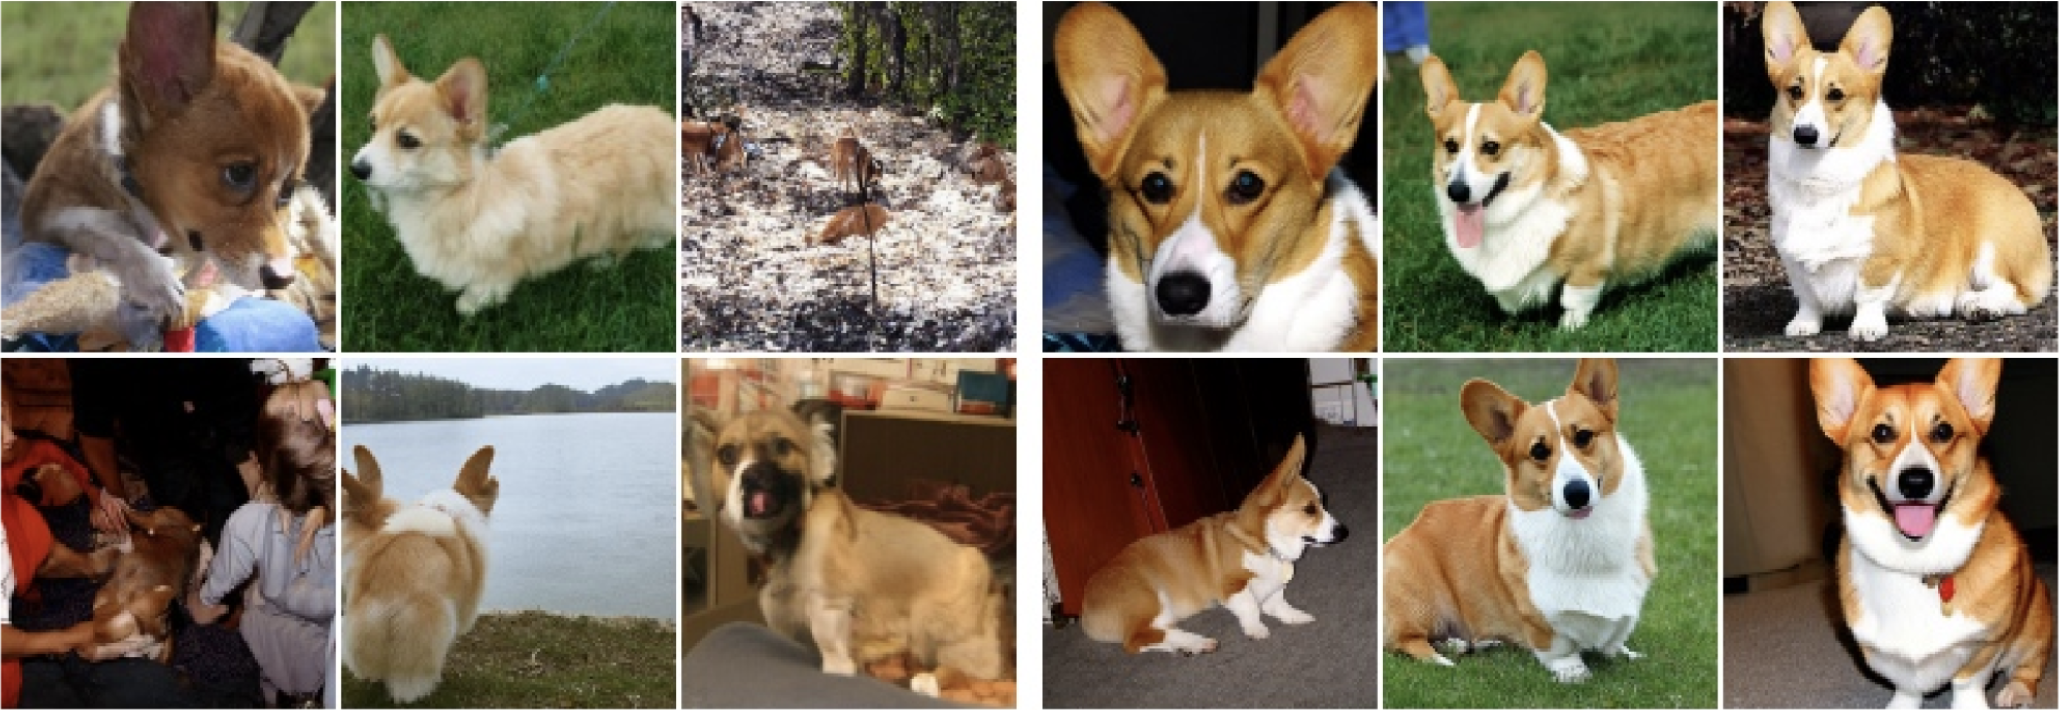
\includegraphics[width=\linewidth]{figures/salimans_cfg.png}
    \caption{The effect of classifier guidance. The prompt here is the "class" chosen to be "Corgi" (a specific type of dog). Left: samples generated with no guidance (i.e., $w = 1$). Right: samples generated with classifier guidance and $w = 4$. As shown, classifier-free guidance improves the similarity to the prompt. Figure taken from \cite{cfg}.分类器指导的效果。这里的提示是选择的"类别"为"柯基犬"(一种特定类型的狗)。左:无指导生成的样本(即$w = 1$)。右:使用分类器指导且$w = 4$生成的样本。如图所示,无分类器指导提高了与提示的相似性。图片来自\cite{cfg}。}
    \label{fig:guidance}
\end{figure}

\begin{figure}[!t]
    \centering
    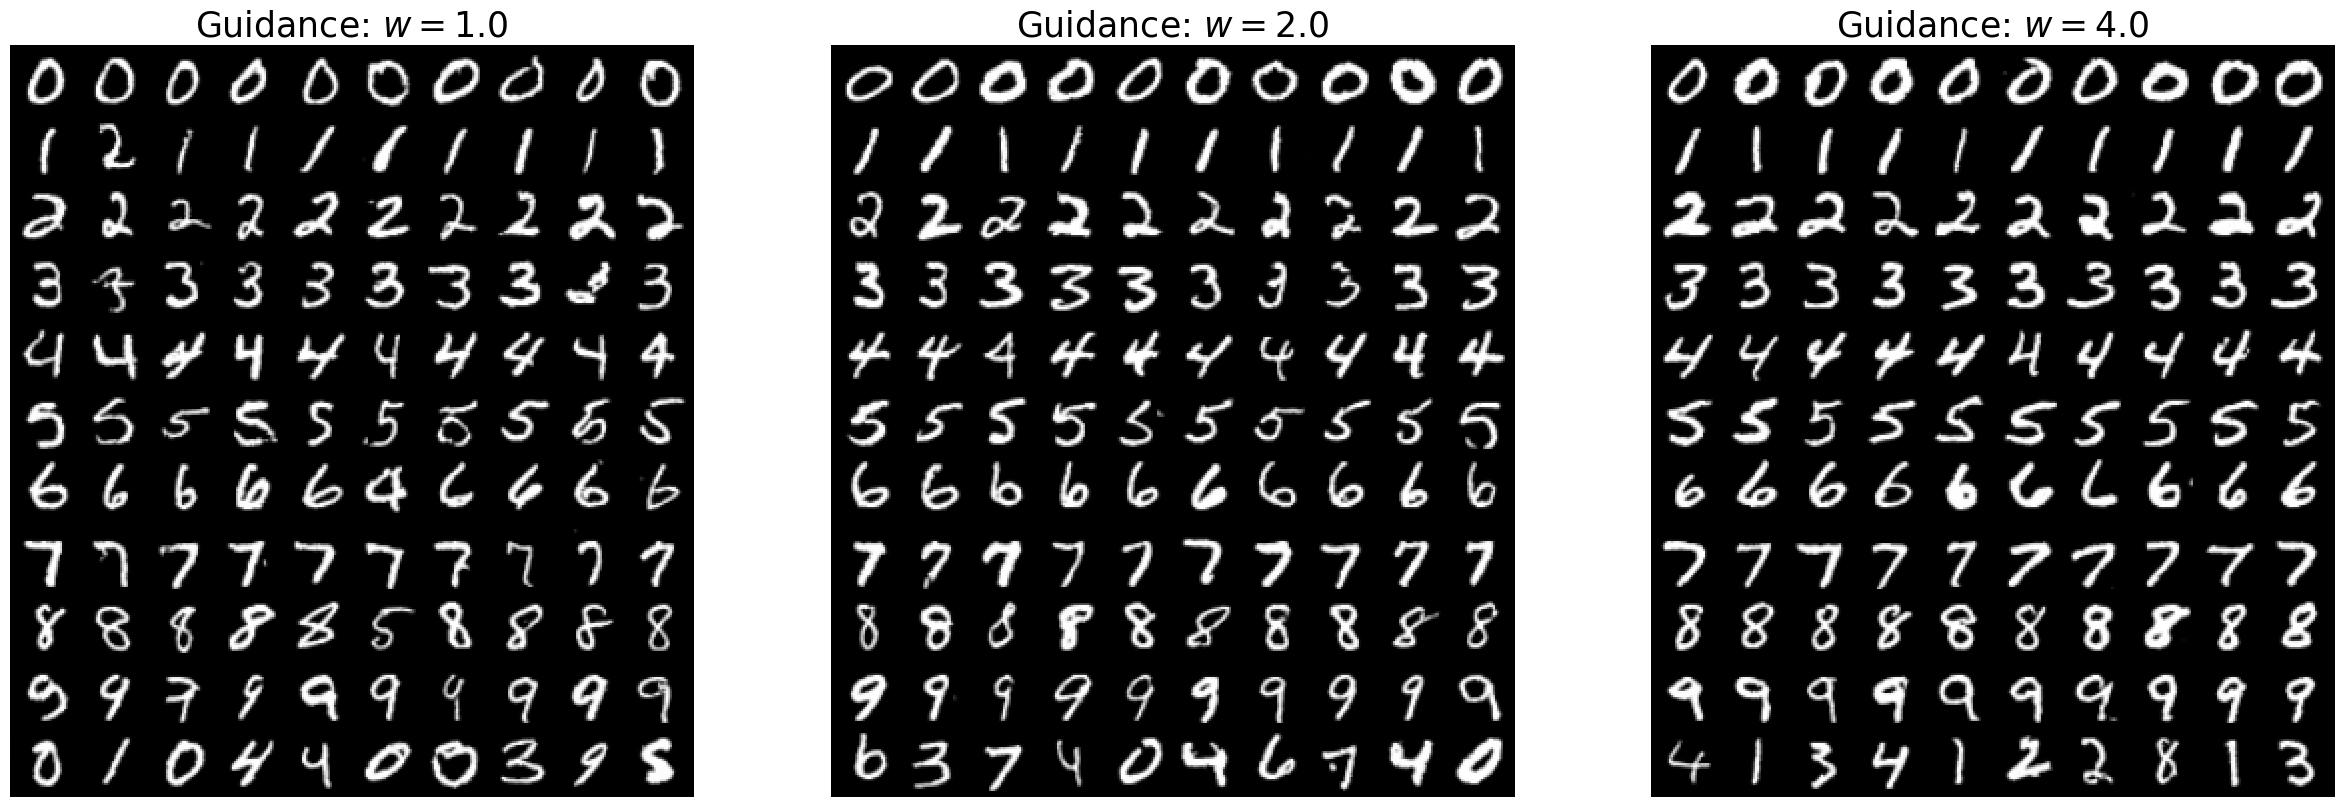
\includegraphics[width=\linewidth]{figures/guidance.png}
    \caption{The effect of classifier-free guidance applied at various guidance scales for the MNIST dataset of hand-written digits. Left: Guidance scale set to $w = 1.0$. Middle: Guidance scale set to $w = 2.0$. Right: Guidance scale set to $w = 4.0$. You will generate a similar image yourself in the lab three!无分类器指导在不同指导尺度下应用于MNIST手写数字数据集的效果。左:指导尺度设置为$w = 1.0$。中:指导尺度设置为$w = 2.0$。右:指导尺度设置为$w = 4.0$。你将在第三个实验中自己生成类似的图像!}
    \label{fig:mnist_guidance}
\end{figure}
In \cref{fig:guidance}, we illustrate class-based classifier-free guidance on 128x128 ImageNet, as in \cite{cfg}. Similarly, in \cref{fig:mnist_guidance}, we visualize the affect of various guidance scales $w$ when applying classifier-free guidance to sampling from the MNIST dataset of handwritten digits.

\begin{algorithm}[h]
\caption{Classifier-free guidance training for Gaussian probability path $p_t(x|z)=\mathcal{N}(x;\alpha_tz,\beta_t^2I_d)$ / 高斯概率路径$p_t(x|z)=\mathcal{N}(x;\alpha_tz,\beta_t^2I_d)$的无分类器引导训练}
\label{alg:training_fm_score_matching_gaussian_paths}
\begin{algorithmic}[1]
\REQUIRE Paired dataset $(z,y)\sim \pdata$, neural network $u_t^\theta$ / 配对数据集$(z,y)\sim \pdata$,神经网络$u_t^\theta$
\FOR{each mini-batch of data / 对于每个数据小批量}
    \STATE Sample a data example $(\dap,y)$ from the dataset. / 从数据集中采样一个数据示例$(\dap,y)$。
    \STATE Sample a random time $t \sim \text{Unif}_{[0,1]}$. / 采样一个随机时间$t \sim \text{Unif}_{[0,1]}$。
    \STATE Sample noise $\epsilon\sim\mathcal{N}(0,I_d)$ / 采样噪声$\epsilon\sim\mathcal{N}(0,I_d)$
    \STATE Set $x=\alpha_t z + \beta_t \epsilon$ / 设置$x=\alpha_t z + \beta_t \epsilon$
    % \hfill (\text{General case: }$x\sim p_t(\cdot|z)$)
    % %\IF{Flow matching}
    \STATE With probability $p$ drop label: $y\leftarrow \varnothing$ / 以概率$p$丢弃标签:$y\leftarrow \varnothing$
    \STATE Compute loss / 计算损失
    \begin{align*}
        \mathcal{L}(\theta) =& \|u_t^\theta(x|y)-(\dot{\alpha}_t\epsilon+\dot{\beta}_tz)\|^2 
    \end{align*}
    \STATE Update the model parameters $\theta$ via gradient descent on $\mathcal{L}(\theta)$. / 通过对$\mathcal{L}(\theta)$进行梯度下降来更新模型参数$\theta$。
\ENDFOR
\end{algorithmic}
\end{algorithm}

\subsubsection{Guidance for Diffusion Models/扩散模型的指导}
In this section we extend the reasoning of the previous section to diffusion models. First, in the same way that we obtained \cref{eq:guided_cfm}, we may generalize the conditional score matching loss \cref{eq:dsm} to obtain the \themebf{guided conditional score matching objective}
\begin{align}
    \label{eq:guided_dsm}
    \mathcal{L}_{\text{CSM}}^{\text{guided}}(\theta) &= \mathbb{E}_{\square}[\|s_t^\theta(x|y) - \nabla\log p_t(x|\dap)\|^2]\\
    \square &= (z,y)\sim \pdata(z,y), \,t\sim \text{Unif},\,x\sim p_t(\cdot|\dap).
\end{align}
A guided score network $s_t^\theta(x|y)$ trained with \cref{eq:guided_dsm} might then be combined with the guided vector field $u_t^\theta(x|y)$ to simulate the SDE
\begin{equation*}
    X_0 \sim \pinit,\quad \dd X_t = \left[u_t^\theta(X_t|y)+\frac{\sigma_t^2}{2}s_t^\theta(X_t|y)\right]\dd t + \sigma_t\dd W_t.
\end{equation*}

在本节中,我们将前一节的推理扩展到扩散模型。首先,与我们获得\cref{eq:guided_cfm}的方式相同,我们可以将条件评分匹配损失\cref{eq:dsm}推广以获得\themebf{引导条件评分匹配目标}
\begin{align}
    \label{eq:guided_dsm}
    \mathcal{L}_{\text{CSM}}^{\text{guided}}(\theta) &= \mathbb{E}_{\square}[\|s_t^\theta(x|y) - \nabla\log p_t(x|\dap)\|^2]\\
    \square &= (z,y)\sim \pdata(z,y), \,t\sim \text{Unif},\,x\sim p_t(\cdot|\dap).
\end{align}
用\cref{eq:guided_dsm}训练的引导评分网络$s_t^\theta(x|y)$然后可以与引导向量场$u_t^\theta(x|y)$结合来仿真SDE
\begin{equation*}
    X_0 \sim \pinit,\quad \dd X_t = \left[u_t^\theta(X_t|y)+\frac{\sigma_t^2}{2}s_t^\theta(X_t|y)\right]\dd t + \sigma_t\dd W_t.
\end{equation*}

\paragraph{Classifier-Free Guidance.} We now extend the classifier-free guidance construction to the diffusion setting. By Bayes' rule (see \cref{eq:bayes_rule}),
\begin{equation*}
    \nabla \log p_t(x|y) = \nabla \log p_t(x) + \nabla \log p_t(y|x),
\end{equation*}
so that for \themebf{guidance scale} $w > 1$ we may define
\begin{align*}
    \tilde{s}_t(x|y) &= \nabla \log p_t(x) + w \nabla \log p_t(y|x)\\
                    &= \nabla \log p_t(x) + w (\nabla \log p_t(x|y) - \nabla \log p_t(x))\\
                    &= (1-w) \nabla \log p_t(x) + w \nabla \log p_t(x|y)\\
                    &= (1-w) \nabla \log p_t(x|\varnothing) + w \nabla \log p_t(x|y)
\end{align*}

\paragraph{无分类器指导。} 现在我们将无分类器指导构造扩展到扩散设置。通过贝叶斯法则(见\cref{eq:bayes_rule}),
\begin{equation*}
    \nabla \log p_t(x|y) = \nabla \log p_t(x) + \nabla \log p_t(y|x),
\end{equation*}
因此对于\themebf{指导尺度}$w > 1$,我们可以定义
\begin{align*}
    \tilde{s}_t(x|y) &= \nabla \log p_t(x) + w \nabla \log p_t(y|x)\\
                    &= \nabla \log p_t(x) + w (\nabla \log p_t(x|y) - \nabla \log p_t(x))\\
                    &= (1-w) \nabla \log p_t(x) + w \nabla \log p_t(x|y)\\
                    &= (1-w) \nabla \log p_t(x|\varnothing) + w \nabla \log p_t(x|y)
\end{align*}
We thus arrive at the CFG-compatible (that is, accounting for the possibility of $\varnothing$) objective 

因此我们得到了CFG兼容的(即考虑$\varnothing$可能性的)目标函数 
\begin{align}
    \label{eq:cfg_guided_dsm}
    \mathcal{L}_{\text{DSM}}^{\text{CFG}}(\theta) &= \,\,\mathbb{E}_{\square} \lVert s_t^{\theta}(x|y) - \nabla \log p_t(x|z)\rVert^2\\
    \square &= (z,y) \sim p_{\text{data}}(z,y),\, t \sim \text{Unif}[0,1),\, x \sim p_t(\cdot|z),\,\text{replace }y=\varnothing\text{ with prob. }\eta,
\end{align}
where $\eta$ is a hyperparameter (the probability of replacing $y$ with $\varnothing$). We will refer $\mathcal{L}_{\text{CSM}}^{\text{CFG}}(\theta)$ as the \themebf{guided conditional score matching objective}. We recap as follows

其中$\eta$是一个超参数(用$\varnothing$替换$y$的概率)。我们将$\mathcal{L}_{\text{CSM}}^{\text{CFG}}(\theta)$称为\themebf{引导条件评分匹配目标}。我们总结如下

\begin{summarybox}[Classifier-Free Guidance for Diffusions/扩散的无分类器指导]
Given the unguided marginal score $\nabla \log p_t(x|\varnothing)$, the guided marginal score field $\nabla \log p_t(x|y)$, and a \themebf{guidance scale} $w > 1$, we define the \themebf{classifier-free guided score} $\tilde{s}_t(x|y)$ by 
\begin{equation}
    \tilde{s}_t(x|y) = (1-w) \nabla \log p_t(x|\varnothing) + w \nabla \log p_t(x|y).
    \label{eq:flow_cfg}
\end{equation}
By approximating $\nabla \log p_t(x|\varnothing)$ and $\nabla \log p_t(x|y)$ using the same neural network $s_t^\theta(x|y)$, we may leverage the following \themebf{classifier-free guidance CSM} (CFG-CSM) objective, given by
\begin{align}
    \label{eq:cfg_guided_dsm}
    \mathcal{L}_{\text{CSM}}^{\text{CFG}}(\theta) &= \,\,\mathbb{E}_{\square} \lVert s_t^{\theta}(x|(1-\xi)y + \xi \varnothing) - \nabla \log p_t(x|z)\rVert^2\\
    \square &= (z,y) \sim p_{\text{data}}(z,y),\, t \sim \text{Unif}[0,1),\, x \sim p_t(\cdot|z),\,\text{replace }y=\varnothing\text{ with prob. }\eta
\end{align}
In plain English, $\mathcal{L}_{\text{DSM}}^{\text{CFG}}$ might be approximated by
\begin{alignat*}{3}
    (z,y) &\sim \pdata(z,y) \quad\quad\quad\quad && \blacktriangleright \quad \text{Sample $(z,y)$ from data distribution.}\\
    t &\sim \text{Unif}[0,1) \quad\quad\quad\quad && \blacktriangleright \quad \text{Sample $t$ uniformly on $[0,1)$.}\\
    x &\sim p_t(x|z,y) \quad\quad\quad\quad && \blacktriangleright \quad \text{Sample $x$ from cond. path $p_t(x|z)$.}\\
    \text{with prob.}&\,\eta,\, y \gets \varnothing \quad\quad\quad\quad && \blacktriangleright \quad \text{Replace $y$ with $\varnothing$ with probability $\eta$.}\\
    \widehat{\mathcal{L}_{\text{DSM}}^{\text{CFG}}}(\theta) &=  \lVert s_t^{\theta}(x|y) - \nabla \log p_t(x|z)\rVert^2 \quad\quad\quad\quad && \blacktriangleright \quad \text{Regress model against conditional score.}
\end{alignat*}
At inference time, for a fixed choice of $w > 1$, we may combine $s_t^\theta(x|y)$ with a guided vector field $u_t^\theta(x|y)$ and define
\begin{align*}
    \tilde{s}^\theta_t(x|y) &= (1-w) s_t^\theta(x|\varnothing) + w s_t^\theta(x|y),\\
    \tilde{u}^\theta_t(x|y) &= (1-w) u_t^\theta(x|\varnothing) + wu_t^\theta (x|y).
\end{align*}
Then we may sample via
\begin{alignat*}{3}
    \textbf{\sffamily Initialization:}\quad X_0&\sim\pinit(x) \quad  && \blacktriangleright\,\,\text{Initialize with simple distribution (such as a Gaussian)}\\
    \textbf{\sffamily Simulation:}\quad \dd X_t &= \left[\tilde{u}_t^\theta(X_t|y)+\frac{\sigma_t^2}{2}\tilde{s}_t^\theta(X_t|y)\right]\dd t + \sigma_t\dd W_t \quad && \blacktriangleright\,\,\text{Simulate SDE from $t=0$ to $t=1$.}\\
    \textbf{\sffamily Samples:}\quad X_1& \quad && \blacktriangleright\,\,\text{Goal is for $X_1$ to adhere to the guiding variable $y$.}
\end{alignat*}

给定无指导边际评分$\nabla \log p_t(x|\varnothing)$、引导边际评分场$\nabla \log p_t(x|y)$和\themebf{指导尺度}$w > 1$,我们通过以下方式定义\themebf{无分类器引导评分}$\tilde{s}_t(x|y)$
\begin{equation}
    \tilde{s}_t(x|y) = (1-w) \nabla \log p_t(x|\varnothing) + w \nabla \log p_t(x|y).
    \label{eq:flow_cfg}
\end{equation}
通过使用相同的神经网络$s_t^\theta(x|y)$近似$\nabla \log p_t(x|\varnothing)$和$\nabla \log p_t(x|y)$,我们可以利用以下\themebf{无分类器指导CSM}(CFG-CSM)目标,由以下给出
\begin{align}
    \label{eq:cfg_guided_dsm}
    \mathcal{L}_{\text{CSM}}^{\text{CFG}}(\theta) &= \,\,\mathbb{E}_{\square} \lVert s_t^{\theta}(x|(1-\xi)y + \xi \varnothing) - \nabla \log p_t(x|z)\rVert^2\\
    \square &= (z,y) \sim p_{\text{data}}(z,y),\, t \sim \text{Unif}[0,1),\, x \sim p_t(\cdot|z),\,\text{replace }y=\varnothing\text{ with prob. }\eta
\end{align}
用通俗的语言,$\mathcal{L}_{\text{DSM}}^{\text{CFG}}$可以通过以下方式近似
\begin{alignat*}{3}
    (z,y) &\sim \pdata(z,y) \quad\quad\quad\quad && \blacktriangleright \quad \text{从数据分布中采样$(z,y)$。}\\
    t &\sim \text{Unif}[0,1) \quad\quad\quad\quad && \blacktriangleright \quad \text{在$[0,1)$上均匀采样$t$。}\\
    x &\sim p_t(x|z,y) \quad\quad\quad\quad && \blacktriangleright \quad \text{从条件路径$p_t(x|z)$中采样$x$。}\\
    \text{以概率}&\,\eta,\, y \gets \varnothing \quad\quad\quad\quad && \blacktriangleright \quad \text{以概率$\eta$将$y$替换为$\varnothing$。}\\
    \widehat{\mathcal{L}_{\text{DSM}}^{\text{CFG}}}(\theta) &=  \lVert s_t^{\theta}(x|y) - \nabla \log p_t(x|z)\rVert^2 \quad\quad\quad\quad && \blacktriangleright \quad \text{将模型与条件评分进行回归。}
\end{alignat*}
在推理时,对于固定选择的$w > 1$,我们可以将$s_t^\theta(x|y)$与引导向量场$u_t^\theta(x|y)$结合并定义
\begin{align*}
    \tilde{s}^\theta_t(x|y) &= (1-w) s_t^\theta(x|\varnothing) + w s_t^\theta(x|y),\\
    \tilde{u}^\theta_t(x|y) &= (1-w) u_t^\theta(x|\varnothing) + wu_t^\theta (x|y).
\end{align*}
然后我们可以通过以下方式采样
\begin{alignat*}{3}
    \textbf{\sffamily 初始化:}\quad X_0&\sim\pinit(x) \quad  && \blacktriangleright\,\,\text{用简单分布(如高斯分布)初始化}\\
    \textbf{\sffamily 仿真:}\quad \dd X_t &= \left[\tilde{u}_t^\theta(X_t|y)+\frac{\sigma_t^2}{2}\tilde{s}_t^\theta(X_t|y)\right]\dd t + \sigma_t\dd W_t \quad && \blacktriangleright\,\,\text{从$t=0$到$t=1$仿真SDE。}\\
    \textbf{\sffamily 样本:}\quad X_1& \quad && \blacktriangleright\,\,\text{目标是使$X_1$遵循指导变量$y$。}
\end{alignat*}
\end{summarybox}

\subsection{Neural network architectures}

\label{sec:image_architecture}
We next discuss the design of neural networks for flow and diffusion models. Specifically, we answer the question of how to construct a neural network architecture that represents the (guided) vector field $u_t^\theta(x|y)$ with parameters $\theta$. Note that the neural network must have 3 inputs - a vector $x\in\R^d$, a conditioning variable $y\in\mathcal{Y}$, and a time value $t\in [0,1]$ - and one output - a vector $u_t^\theta(x|y)\in\mathbb{R}^d$. For low-dimensional distributions (e.g. the toy distributions we have seen in previous sections), it is sufficient to parameterize $u_t^\theta(x|y)$ as a multi-layer perceptron (MLP), otherwise known as a fully connected neural network. That is, in this simple setting, a forward pass through $u_t^\theta(x|y)$ would involve concatenating our input $x$, $y$, and $t$, and passing them through an MLP. However, for complex, high-dimensional distributions, such as those over images, videos, and proteins, an MLP is rarely sufficient, and it is common to use special, application-specific architectures. For the remainder of this section, we will consider the case of \textbf{images} (and by extension, videos), and discuss two common architectures: the \themebf{U-Net} \citep{ronneberger2015u}, and the \themebf{diffusion transformer} (DiT).\\

\label{sec:image_architecture}
接下来我们讨论流模型和扩散模型的神经网络设计。具体来说,我们回答如何构造一个神经网络架构来表示带参数$\theta$的(引导)向量场$u_t^\theta(x|y)$的问题。注意神经网络必须有3个输入——向量$x\in\R^d$、条件变量$y\in\mathcal{Y}$和时间值$t\in [0,1]$——以及一个输出——向量$u_t^\theta(x|y)\in\mathbb{R}^d$。对于低维分布(例如我们在前面章节中看到的玩具分布),将$u_t^\theta(x|y)$参数化为多层感知机(MLP),也称为全连接神经网络,是足够的。也就是说,在这种简单设置中,通过$u_t^\theta(x|y)$的前向传递将涉及连接我们的输入$x$、$y$和$t$,并将它们通过MLP。然而,对于复杂的高维分布,例如图像、视频和蛋白质上的分布,MLP很少足够,通常使用特殊的、应用特定的架构。在本节的其余部分,我们将考虑\textbf{图像}(并扩展到视频)的情况,并讨论两种常见架构:\themebf{U-Net} \citep{ronneberger2015u}和\themebf{扩散变换器}(DiT)。\\

\subsubsection{U-Nets and Diffusion Transformers}
Before we dive into the specifics of these architectures, let us recall from the introduction that an image is simply a vector $x \in \mathbb{R}^{C_{\text{image}} \times H \times W}$. Here $C_{\text{image}}$ denotes the number of \themebf{channels} (an RGB image typically would have $C_{\text{input}} = 3$ color channels), $H$ denotes the \themebf{height} of the image in pixels, and $W$ denotes the \themebf{width} of the image in pictures. %As we will soon see with the U-Net, the channel dimension is often used as a means to introduce deeper, latent features. 

在我们深入了解这些架构的细节之前,让我们回忆一下引言中提到的,图像简单地是一个向量$x \in \mathbb{R}^{C_{\text{image}} \times H \times W}$。这里$C_{\text{image}}$表示\themebf{通道}数(RGB图像通常有$C_{\text{input}} = 3$个颜色通道),$H$表示图像的\themebf{高度}(以像素为单位),$W$表示图像的\themebf{宽度}(以像素为单位)。%正如我们很快会看到的U-Net,通道维度经常被用作引入更深层潜在特征的手段。

\paragraph{U-Nets.} The \themebf{U-Net} architecture \citep{ronneberger2015u} is a specific type of convolutional neural network. Originally designed for image segmentation, its crucial feature is that both its input and its output have the shape of images (possibly with a different number of channels). This makes it ideal to parameterize a vector field $x\mapsto u_t^\theta(x|y)$ as for fixed $y,t$ its input has the shape of an image and its output does, too. Therefore, U-Net were widely used in the development of diffusion models. A U-Net consists of a series of \themebf{encoders} $\mathcal{E}_i$, and a corresponding sequence of \themebf{decoders} $\mathcal{D}_i$, along with a latent processing block in between, which we shall refer to as a \themebf{midcoder} (midcoder is a term is not used in the literature usually). For sake of example, let us walk through the path taken by an image $x_t \in \mathbb{R}^{3 \times 256 \times 256}$ (we have taken $(C_{\text{input}}, H, W) = (3, 256, 256)$) as it is processed by the U-Net:
\paragraph{U-Net。} \themebf{U-Net}架构\citep{ronneberger2015u}是一种特定类型的卷积神经网络。最初为图像分割设计,其关键特征是其输入和输出都具有图像的形状(可能具有不同数量的通道)。这使得它非常适合参数化向量场$x\mapsto u_t^\theta(x|y)$,因为对于固定的$y,t$,其输入具有图像的形状,其输出也是如此。因此,U-Net在扩散模型的发展中被广泛使用。U-Net由一系列\themebf{编码器}$\mathcal{E}_i$和相应的\themebf{解码器}$\mathcal{D}_i$序列组成,以及中间的潜在处理块,我们称之为\themebf{中间编码器}(中间编码器这个术语在文献中通常不使用)。作为例子,让我们走过图像$x_t \in \mathbb{R}^{3 \times 256 \times 256}$(我们取$(C_{\text{input}}, H, W) = (3, 256, 256)$)在U-Net中处理的路径:

\begin{alignat*}{3}
    x^{\text{input}}_t &\in \mathbb{R}^{3 \times 256 \times 256} \quad  
    && \blacktriangleright\,\,\text{Input to the U-Net.}\\
    x^{\text{latent}}_t = \mathcal{E}(x^{\text{input}}_t) &\in \mathbb{R}^{512 \times 32 \times 32} \quad && \blacktriangleright\,\,\text{Pass through encoders to obtain latent.}\\
    x^{\text{latent}}_t = \mathcal{M}(x^{\text{latent}}_t) &\in \mathbb{R}^{512 \times 32 \times 32} \quad && \blacktriangleright\,\,\text{Pass latent through midcoder.}\\
    x^{\text{output}}_t = \mathcal{D}(x^{\text{latent}}_t) &\in \mathbb{R}^{3 \times 256 \times 256} \quad && \blacktriangleright\,\,\text{Pass through decoders to obtain output.}
\end{alignat*}
Notice that as the input passes through the encoders, the number of channels in its representation increases, while the height and width of the images are decreased. Both the encoder and the decoder usually consist of a series of convolutional layers (with activation functions, pooling operations, etc. in between). Not shown above are two points: First, the input $x^{\text{input}}_t\in \mathbb{R}^{3 \times 256 \times 256}$ is often fed into an initial pre-encoding block to increase the number of channels before being fed into the first encoder block. Second, the encoders and decoders are often connected by \themebf{residual connections}. The complete picture is shown in \cref{fig:unet}.

注意,当输入通过编码器时,其表示中的通道数增加,而图像的高度和宽度减少。编码器和解码器通常都由一系列卷积层组成(中间有激活函数、池化操作等)。上面没有显示的有两点:首先,输入$x^{\text{input}}_t\in \mathbb{R}^{3 \times 256 \times 256}$通常被馈送到初始预编码块中,以在馈送到第一个编码器块之前增加通道数。其次,编码器和解码器经常通过\themebf{残差连接}连接。完整的图片如\cref{fig:unet}所示。

\begin{figure}
    \centering
    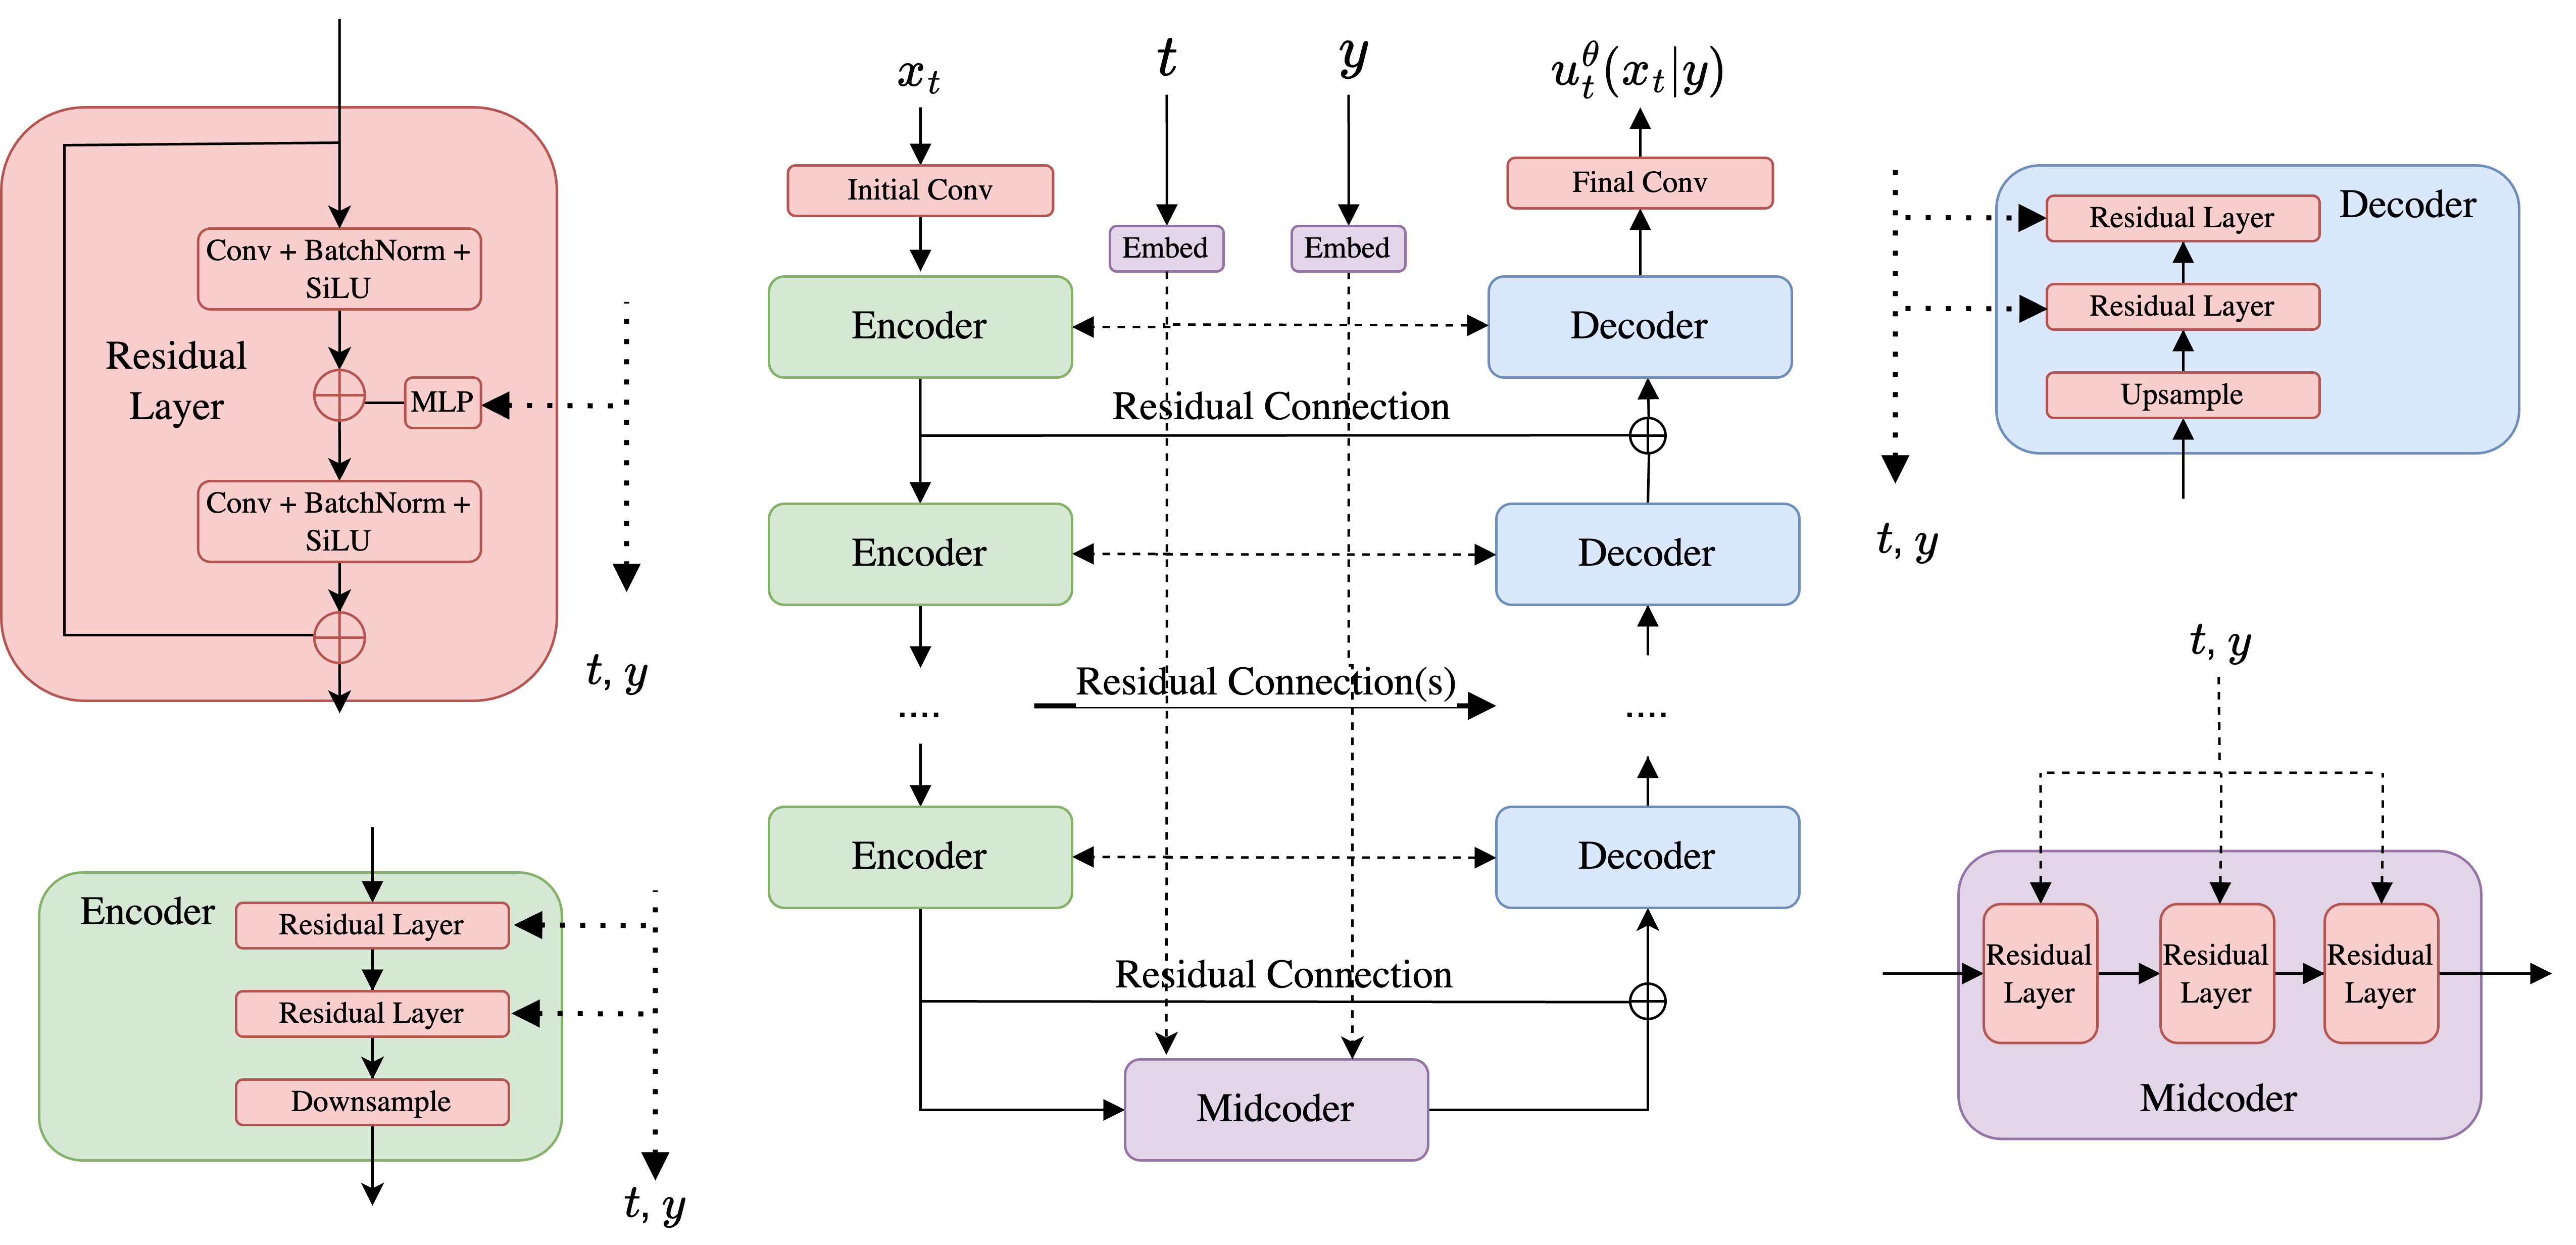
\includegraphics[width=\textwidth]{figures/unet.png}
    \caption{The simplified U-Net architecture used in lab three./实验三中使用的简化U-Net架构。}
    \label{fig:unet}
\end{figure}


At a high level, most U-Nets involve some variant of what is described above. However, certain of the design choices described above may well differ from various implementations in practice. In particular, we opt above for a purely-convolutional architecture whereas it is common to include attention layers as well throughout the encoders and decoders. The U-Net derives its name from the ``U''-like shape formed by its encoders and decoders (see \cref{fig:unet}).

在高层次上,大多数U-Net都涉及上述描述的某种变体。然而,上述描述的某些设计选择在实践中的各种实现中可能会有所不同。特别是,我们在上面选择了纯卷积架构,而在编码器和解码器中包含注意力层也是常见的。U-Net的名称来源于其编码器和解码器形成的"U"形形状(见\cref{fig:unet})。

\paragraph{Diffusion Transformers.} One alternative to U-Nets are \themebf{diffusion transformers} (DiTs), which dispense with convolutions and purely use \themebf{attention} \cite{attention, dit}. Diffusion transformers are based on \themebf{vision transformers} (ViTs), in which the big idea is essentially to divide up an image into patches, embed each of these patches, and then attend between the patches \cite{vit}. \themeit{Stable Diffusion 3}, trained with conditional flow matching, parameterizes the velocity field $u_t^{\theta}(x)$ as a modified DiT, as we discuss later in \cref{sec:large_scale_models} \cite{sd3}.

\paragraph{扩散变换器。} U-Net的一种替代方案是\themebf{扩散变换器}(DiT),它们摒弃了卷积,纯粹使用\themebf{注意力}\cite{attention, dit}。扩散变换器基于\themebf{视觉变换器}(ViT),其中的主要思想本质上是将图像分割成补丁,嵌入每个补丁,然后在补丁之间进行注意力计算\cite{vit}。用条件流匹配训练的\themeit{Stable Diffusion 3}将速度场$u_t^{\theta}(x)$参数化为修改的DiT,我们稍后在\cref{sec:large_scale_models}中讨论\cite{sd3}。

\begin{remarkbox}[Working in Latent Space/在潜在空间中工作]
A common problem for large-scale applications is that the data is so high-dimensional that it consumes too much memory. For example, we might want to generate a high resolution image of $1000\times 10000$ pixels leading to $1$ million (!) dimensions. To reduce memory usage, a common design pattern is to work in a \themebf{latent space} that can be considered a compressed version of our data at lower resolution.  Specifically, the usual approach is to combine a flow or diffusion model with a (variational) \themebf{autoencoder} \cite{latent_diffusion}. In this case, one first encodes the training dataset in the \themebf{latent space} via an autoencoder, and then training the flow or diffusion model in the latent space. Sampling is performed by first sampling in the latent space using the trained flow or diffusion model, and then decoding of the output via the decoder. Intuitively, a well-trained autoencoder can be thought of as filtering out semantically meaningless details, allowing the generative model to ``focus'' on important, perceptually relevant features \cite{latent_diffusion}. By now, nearly all state-of-the-art approaches to image and video generation involve training a flow or diffusion model in the latent space of an autoencoder - so called \themebf{latent diffusion models} \citep{latent_diffusion,vahdat2021score}. However, it is important to note: one also needs to train the autoencoder before training the diffusion models. Crucially, performance now depends also on how good the autoencoder compresses images into latent space and recovers aesthetically pleasing images.

大规模应用的一个常见问题是数据的维度太高,消耗太多内存。例如,我们可能想要生成$1000\times 10000$像素的高分辨率图像,导致$1$百万(!)维度。为了减少内存使用,一种常见的设计模式是在\themebf{潜在空间}中工作,该空间可以被视为我们在较低分辨率下的数据的压缩版本。具体而言,通常的方法是将流模型或扩散模型与(变分)\themebf{自编码器}结合\cite{latent_diffusion}。在这种情况下,首先通过自编码器在\themebf{潜在空间}中编码训练数据集,然后在潜在空间中训练流模型或扩散模型。采样通过首先使用训练的流模型或扩散模型在潜在空间中采样,然后通过解码器解码输出来执行。直观地,一个训练良好的自编码器可以被认为是过滤掉语义上无意义的细节,允许生成模型"专注"于重要的、感知相关的特征\cite{latent_diffusion}。到现在,几乎所有最先进的图像和视频生成方法都涉及在自编码器的潜在空间中训练流模型或扩散模型——所谓的\themebf{潜在扩散模型}\citep{latent_diffusion,vahdat2021score}。然而,重要的是要注意:在训练扩散模型之前,还需要训练自编码器。关键的是,性能现在也取决于自编码器将图像压缩到潜在空间并恢复美观图像的效果如何。
\end{remarkbox}

\subsubsection{Encoding the Guiding Variable.} 
Up until this point, we have glossed over how exactly the guiding (conditioning) variable $y$ is fed into the neural network $u_t^\theta(x|y)$. Broadly, this process can be decomposed into two steps: embedding the raw input $y_{\text{raw}}$ (e.g., the text prompt ``a cat playing a trumpet, photorealistic'') into some vector-valued input $y$, and feeding the resulting $y$ into the actual model. We now proceed to describe each step in greater detail.

到目前为止,我们忽略了引导(条件)变量$y$如何准确地被馈送到神经网络$u_t^\theta(x|y)$中。广义上,这个过程可以分解为两个步骤:将原始输入$y_{\text{raw}}$(例如,文本提示"一只猫在吹小号,照片真实感")嵌入到某个向量值输入$y$中,以及将结果$y$馈送到实际模型中。我们现在更详细地描述每个步骤。

\paragraph{Embedding Raw Input.} Here, we'll consider two cases: (1) where $y_{\text{raw}}$ is a discrete class-label, and (2) where $y_{\text{raw}}$ is a text-prompt. When $y_{\text{raw}} \in \mathcal{Y} \triangleq \{0,\dots, N\}$ is just a class label, then it is often easiest to simply learn a separate embedding vector for each of the $N+1$ possible values of $y_{\text{raw}}$, and set $y$ to this embedding vector. One would consider the parameters of these embeddings to be included in the parameters of $u_t^\theta(x|y)$, and would therefore learn these during training. When $y_{\text{raw}}$ is a text-prompt, the situation is more complex, and approaches largely rely on frozen, pre-trained models. Such models are trained to embed a discrete text input into a continuous vector that captures the relevant information. One such model is known as \themebf{CLIP} (Contrastive Language-Image Pre-training). CLIP is trained to learn a shared embedding space for both images and text-prompts, using a training loss designed to encourage image embeddings to be close to their corresponding prompts, while being farther from the embeddings of other images and prompts \cite{clip}. We might therefore take $y = \text{CLIP}(y_{\text{raw}}) \in \mathbb{R}^{d_{\text{CLIP}}}$ to be the embedding produced by a frozen, pre-trained CLIP model. In certain cases, it may be undesirable to compress the entire sequence into a single representation. In this case, one might additionally consider embedding the prompt using a pre-trained transformer so as to obtain a sequence of embeddings. It is also common to combine multiple such pretrained embeddings when conditioning so as to simultaneously reap the benefits of each model \cite{sd3, moviegen}.

\paragraph{嵌入原始输入。} 在这里,我们将考虑两种情况:(1)$y_{\text{raw}}$是离散类标签,(2)$y_{\text{raw}}$是文本提示。当$y_{\text{raw}} \in \mathcal{Y} \triangleq \{0,\dots, N\}$只是一个类标签时,通常最简单的方法是为$y_{\text{raw}}$的$N+1$个可能值中的每一个简单地学习一个单独的嵌入向量,并将$y$设置为此嵌入向量。我们将这些嵌入的参数视为包含在$u_t^\theta(x|y)$的参数中,因此将在训练期间学习这些参数。当$y_{\text{raw}}$是文本提示时,情况更复杂,方法主要依赖于冻结的预训练模型。这些模型被训练来将离散文本输入嵌入到捕获相关信息的连续向量中。一个这样的模型被称为\themebf{CLIP}(对比语言-图像预训练)。CLIP被训练来学习图像和文本提示的共享嵌入空间,使用旨在鼓励图像嵌入接近其对应提示的训练损失,同时远离其他图像和提示的嵌入\cite{clip}。因此,我们可以取$y = \text{CLIP}(y_{\text{raw}}) \in \mathbb{R}^{d_{\text{CLIP}}}$作为由冻结的预训练CLIP模型产生的嵌入。在某些情况下,将整个序列压缩为单个表示可能是不希望的。在这种情况下,可以另外考虑使用预训练变换器嵌入提示,以获得嵌入序列。在条件化时结合多个这样的预训练嵌入也是常见的,以便同时获得每个模型的好处\cite{sd3, moviegen}。

\begin{figure}[!t]
\centering
\begin{subfigure}{.5\textwidth}
  \centering
  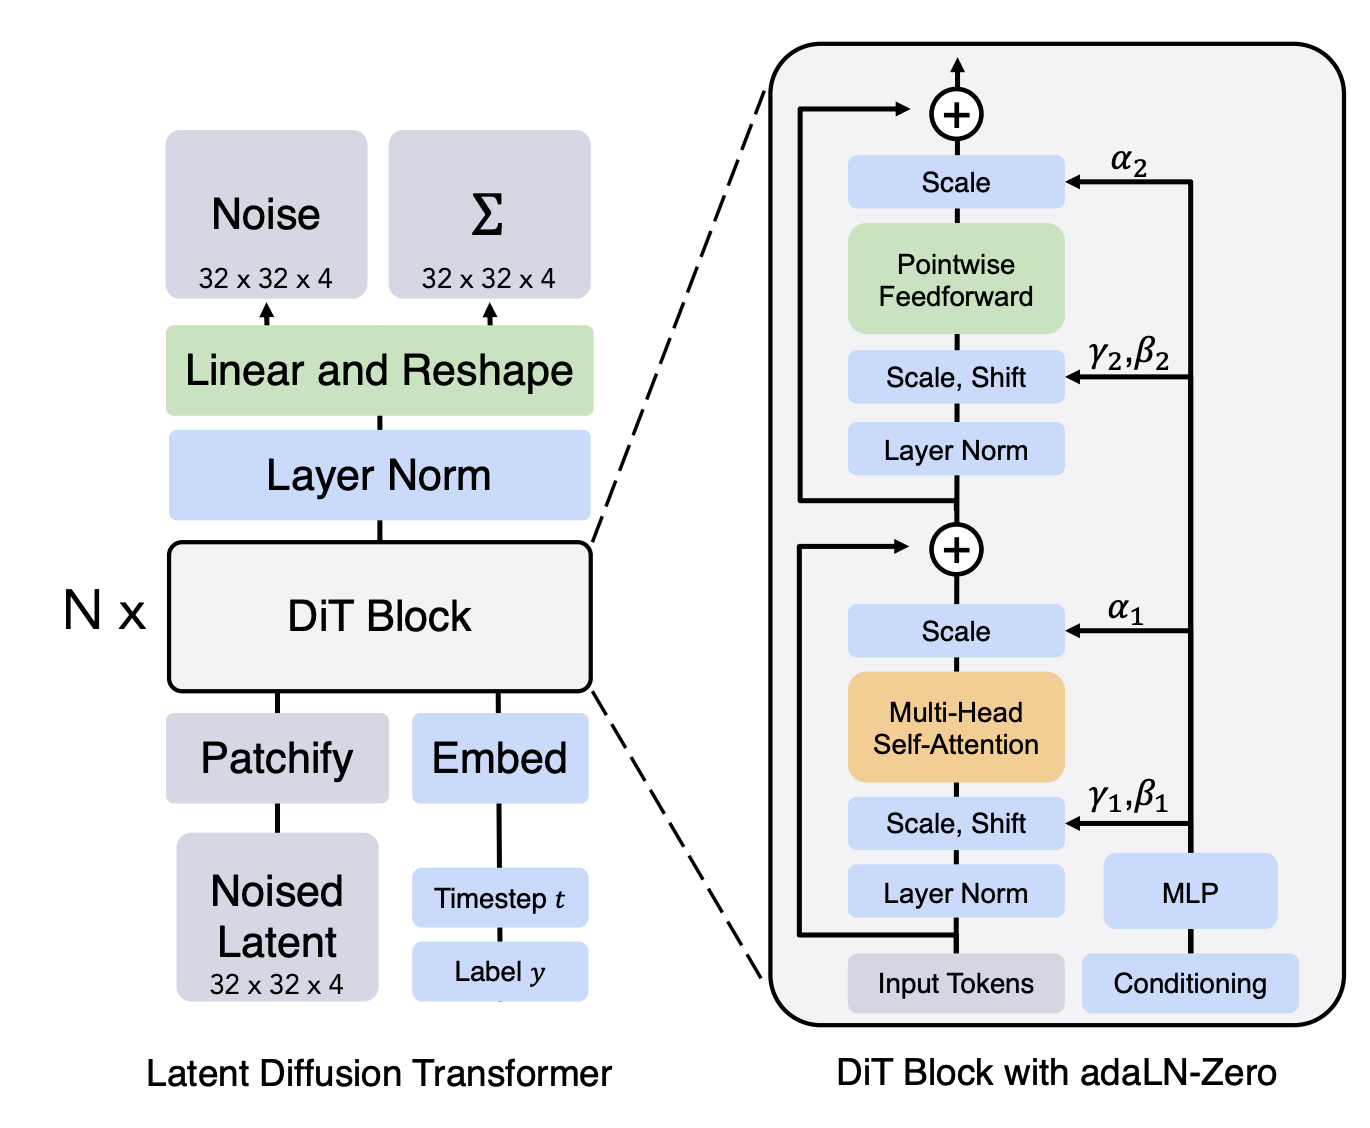
\includegraphics[width=0.95\linewidth]{figures/dit.png}
  \label{fig:sub1}
\end{subfigure}%
\begin{subfigure}{.5\textwidth}
  \centering
  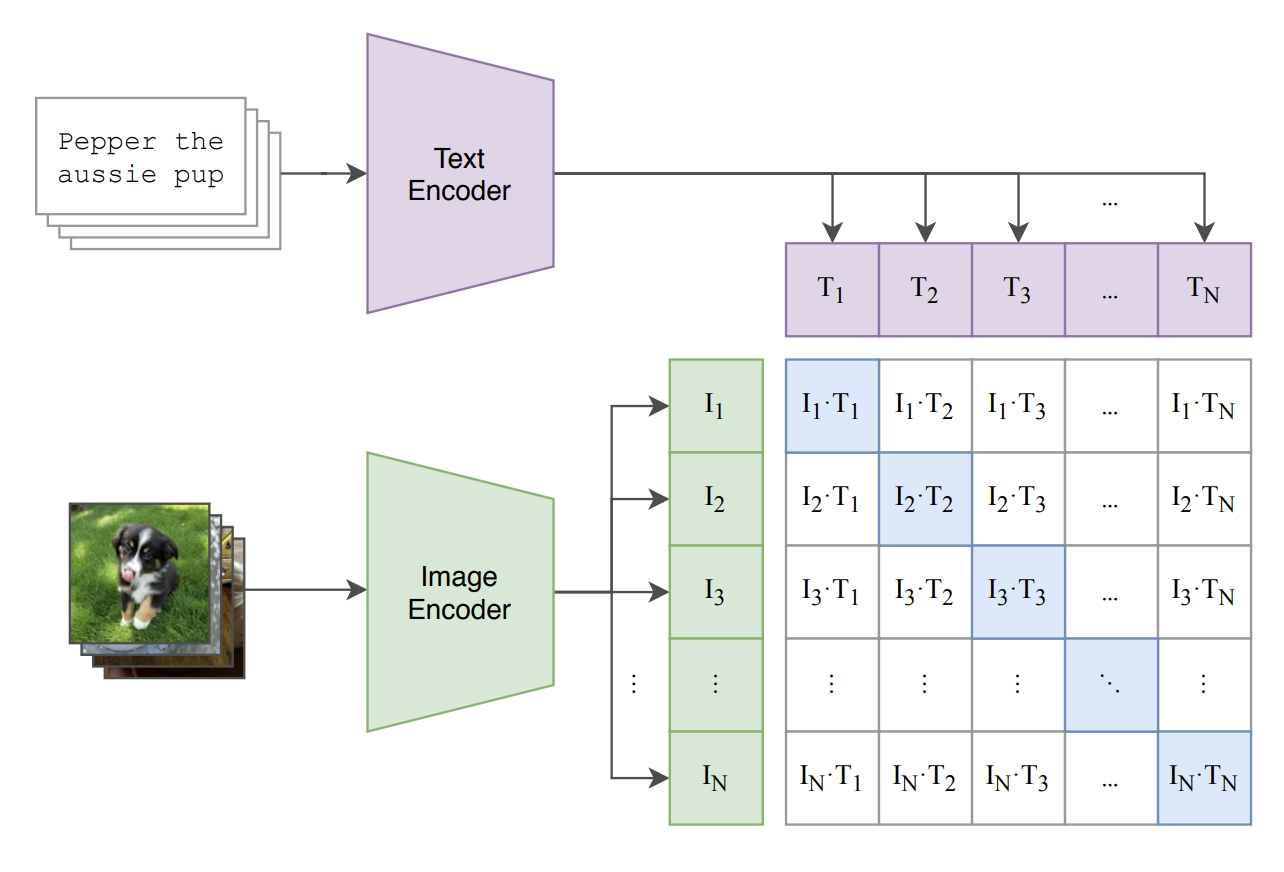
\includegraphics[width=0.95\linewidth]{figures/clip.png}
  \label{fig:sub2}
\end{subfigure}
\caption{Left: An overview of the diffusion transformer architecture, taken from \cite{dit}. Right: A schematic of the contrastive CLIP loss, in which a shared image-text embedding space is learned, taken from \cite{clip}.左:扩散变换器架构概述,取自\cite{dit}。右:对比CLIP损失示意图,其中学习了共享图像-文本嵌入空间,取自\cite{clip}。}
\label{fig:test}
\end{figure}


\paragraph{Feeding in the Embedding.} Suppose now that we have obtained our embedding vector $y \in \mathbb{R}^{d_y}$. Now what? The answer varies, but usually it is some variant of the following: feed it individually into every sub-component of the architecture for images. Let us briefly describe how this is accomplished in the U-Net implementation used in lab three, as depicted in \cref{fig:unet}. At some intermediate point within the network, we would like to inject information from $y \in \mathbb{R}^{d_y}$ into the current activation $x^{\text{intermediate}}_t \in \mathbb{R}^{C \times H \times W}$. We might do so using the procedure below, given in PyTorch-esque pseudocode.

\begin{align*}
    y &= \text{MLP}(y) \in \mathbb{R}^C\quad 
    && \blacktriangleright\,\,\text{Map $y$ from $\mathbb{R}^{d_y}$ to $\mathbb{R}^C$.}\\
    y &= \text{reshape}(y) \in \mathbb{R}^{C \times 1 \times 1}\quad 
    && \blacktriangleright\,\,\text{Reshape $y$ to ``look'' like an image.}\\
    x^{\text{intermediate}}_t &= \text{broadcast\_add}(x^{\text{intermediate}}_t,y) \in \mathbb{R}^{C \times H \times W}\quad && \blacktriangleright\,\,\text{Add $y$ to $x^{\text{intermediate}}_t$ pointwise.}
\end{align*}

One exception to this simple-pointwise conditioning scheme is when we have a sequence of embeddings as produced by some pretrained language model. In this case, we might consider using some sort of cross-attention scheme between our image (suitably patchified) and the tokens of the embedded sequence. We will see multiple examples of this in \cref{sec:large_scale_models}.

\paragraph{馈入嵌入。} 现在假设我们已经获得了嵌入向量$y \in \mathbb{R}^{d_y}$。现在怎么办?答案各不相同,但通常是以下的某种变体:将其单独馈入图像架构的每个子组件。让我们简要描述如何在实验三中使用的U-Net实现中完成这一点,如\cref{fig:unet}所示。在网络内的某个中间点,我们希望将来自$y \in \mathbb{R}^{d_y}$的信息注入到当前激活$x^{\text{intermediate}}_t \in \mathbb{R}^{C \times H \times W}$中。我们可以使用下面的过程来做到这一点,以类似PyTorch的伪代码给出。

\begin{align*}
    y &= \text{MLP}(y) \in \mathbb{R}^C\quad 
    && \blacktriangleright\,\,\text{将$y$从$\mathbb{R}^{d_y}$映射到$\mathbb{R}^C$。}\\
    y &= \text{reshape}(y) \in \mathbb{R}^{C \times 1 \times 1}\quad 
    && \blacktriangleright\,\,\text{重塑$y$使其"看起来"像图像。}\\
    x^{\text{intermediate}}_t &= \text{broadcast\_add}(x^{\text{intermediate}}_t,y) \in \mathbb{R}^{C \times H \times W}\quad && \blacktriangleright\,\,\text{将$y$逐点添加到$x^{\text{intermediate}}_t$。}
\end{align*}

这种简单逐点条件化方案的一个例外是当我们有由某些预训练语言模型产生的嵌入序列时。在这种情况下,我们可能考虑在我们的图像(适当分块)和嵌入序列的标记之间使用某种交叉注意力方案。我们将在\cref{sec:large_scale_models}中看到多个这样的例子。

\subsection{A Survey of Large-Scale Image and Video Models}

\label{sec:large_scale_models}
We conclude this section by briefly examining two large-scale generative models: \themeit{Stable Diffusion 3} for image generation and Meta's \themeit{Movie Gen Video} for video generation \citep{sd3, moviegen}. As you will see, these models use the techniques we have described in this work along with additional architectural enhancements to both scale and accommodate richly structured conditioning modalities, such as text-based input.

大规模图像和视频模型调研

我们通过简要研究两个大规模生成模型来结束本节:用于图像生成的\themeit{Stable Diffusion 3}和Meta的用于视频生成的\themeit{Movie Gen Video} \citep{sd3, moviegen}。正如您将看到的,这些模型使用了我们在本工作中描述的技术,同时还增加了额外的架构增强功能,以便扩展和适应丰富结构化的条件模态,如基于文本的输入。

\subsubsection{Stable Diffusion 3}

Stable Diffusion is a series of state-of-the-art image generation models. These models were among the first to use large-scale latent diffusion models for image generation. If you have not done so, we highly recommend testing it for yourself online (\url{https://stability.ai/news/stable-diffusion-3}).\\


Stable Diffusion是一系列最先进的图像生成模型。这些模型是首批使用大规模潜在扩散模型进行图像生成的模型之一。如果您还没有这样做,我们强烈建议您在线亲自测试(\url{https://stability.ai/news/stable-diffusion-3})。\\

%\paragraph{Training Objective.} 
Stable Diffusion 3 uses the same conditional flow matching objective that we study in this work (see \cref{alg:training_fm_score_matching_gaussian_paths}).\footnote{In their work, they use a different convention to condition on the noise. But this is only notation and the algorithm is the same.} As outlined in their paper, they extensively tested various flow and diffusion alternatives and found flow matching to perform best. For training, it uses classifier-free guidance training (with dropping class labels) as outlined above. Further, Stable Diffusion 3 follows the approach outlined in \cref{sec:image_architecture} by training within the latent space of a pre-trained autoencoder. Training a good autoencoder was a big contribution of the first stable diffusion papers.\\

%\paragraph{Training Objective.} 
Stable Diffusion 3使用我们在本工作中研究的相同条件流匹配目标(见\cref{alg:training_fm_score_matching_gaussian_paths})。\footnote{在他们的工作中,他们使用不同的约定来条件化噪声。但这只是符号,算法是相同的。}正如他们论文中概述的,他们广泛测试了各种流和扩散替代方案,发现流匹配表现最好。对于训练,它使用如上所述的无分类器指导训练(丢弃类标签)。此外,Stable Diffusion 3遵循\cref{sec:image_architecture}中概述的方法,在预训练自编码器的潜在空间内进行训练。训练一个好的自编码器是第一批稳定扩散论文的重大贡献。\\

To enhance text conditioning, Stable Diffusion 3 makes use of both 3 different types of text embeddings (including CLIP embeddings as well as the sequential outputs produced by a pretrained instance of the encoder of Google's T5-XXL \cite{t5}, and similar to approaches taken in \cite{balaji, saharia}). Whereas CLIP embeddings provide a coarse, overarching embedding of the input text, the T5 embeddings provide a more granular level of context, allowing for the possibility of the model attending to particular elements of the conditioning text. To accommodate these sequential context embeddings, the authors then propose to extend the diffusion transformer to attend not just to patches of the image, but to the text embeddings as well, thereby extending the conditioning capacity from the class-based scheme originally proposed for DiT to sequential context embeddings. This proposed modified DiT is referred to as a \themebf{multi-modal DiT} (MM-DiT), and is depicted in \cref{fig:mmdit}. Their final, largest model has \textbf{8 billion parameters}. For sampling, they use $50$ steps (i.e. they have to evaluate the network $50$ times) using a Euler simulation scheme and a classifier-free guidance weight between $2.0$-$5.0$.

为了增强文本条件化,Stable Diffusion 3使用了3种不同类型的文本嵌入(包括CLIP嵌入以及由Google的T5-XXL编码器的预训练实例产生的序列输出\cite{t5},类似于\cite{balaji, saharia}中采用的方法)。虽然CLIP嵌入提供了输入文本的粗略、全面的嵌入,但T5嵌入提供了更细粒度的上下文级别,允许模型关注条件文本的特定元素。为了适应这些序列上下文嵌入,作者然后提议扩展扩散变换器,不仅关注图像的补丁,还关注文本嵌入,从而将条件化能力从最初为DiT提议的基于类的方案扩展到序列上下文嵌入。这个提议的修改DiT被称为\themebf{多模态DiT}(MM-DiT),如\cref{fig:mmdit}所示。他们最终的最大模型有\textbf{80亿参数}。对于采样,他们使用$50$步(即他们必须评估网络$50$次),使用欧拉仿真方案和$2.0$-$5.0$之间的无分类器指导权重。
% \begin{equation}
% \label{eq:sd3_cfm}
% \begin{aligned}
%     \Lcond(\theta) &=  \mathbb{E}_{\square}[\|u_t^\theta(x_t) - \uref_t(x_t|\varepsilon)\|^2]\\
%     \square &= \varepsilon \sim \mathcal{N}(0, I_d), x_t\sim p_t(\cdot|\varepsilon)
% \end{aligned}
% \end{equation}
% where $p_0 = \mathcal{N}(0, I_d)$. 
% Note that \cref{eq:sd3_cfm} differs from \cref{eq:cfm} in that we condition on $\varepsilon \in p_0 = \mathcal{N}(0,I_d)$ rather than $z \in p_{\text{data}}$. The analysis is otherwise fundamentally the same. Here, the conditional probability path $p_t(\cdot | \varepsilon)$ is defined implicitly as the law of the random variable
% \begin{equation}
%     X_t \triangleq \alpha_tX_1 + \beta_t \varepsilon, \quad \quad X_1 \sim p_{\text{data}},
% \end{equation}
% where $\alpha_t,\beta_t \in \mathcal{C}^2([0,1])$ satisfy $\alpha_0 = \beta_1 = 0$ and $\alpha_1 = \beta_0 = 1$ \cite{albergo2023stochastic}. Then, \cref{eq:sd3_cfm} may be modified to the general conditional setting as in \cref{eq:cfg_guided_cfm}.

\begin{figure}[!t]
    \centering
    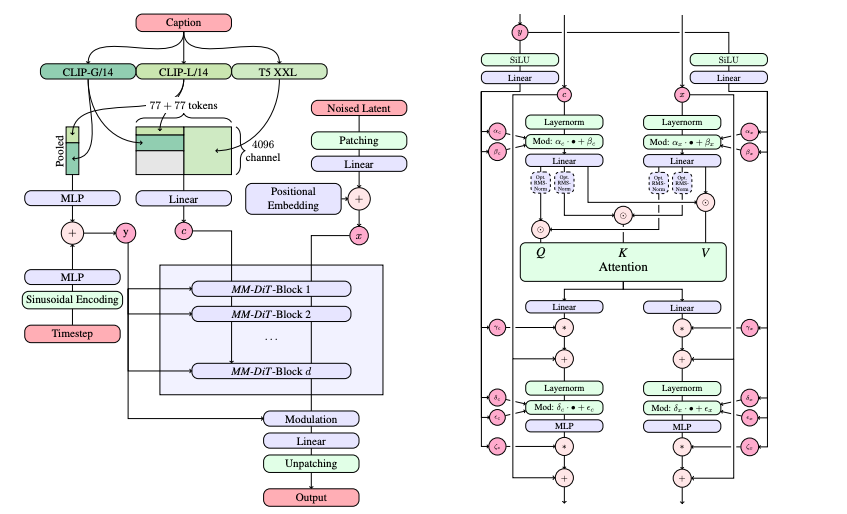
\includegraphics[width=0.9\textwidth]{figures/mmdit.png}
    \caption{The architecture of the multi-modal diffusion transformer (MM-DiT) proposed in \citep{sd3}. Figure also taken from \citep{sd3}.\citep{sd3}中提出的多模态扩散变换器(MM-DiT)的架构。图也取自\citep{sd3}。}
    \label{fig:mmdit}
\end{figure}


%\paragraph{Architecture.}

\subsubsection{Meta Movie Gen Video}
Next, we discuss Meta's video generator, \themeit{Movie Gen Video} (\url{https://ai.meta.com/research/movie-gen/}). As the data are not images but \themeit{videos},  the data $x$ lie in the space $\mathbb{R}^{T \times C \times H \times W}$ where $T$ represents the new \themebf{temporal} dimension (i.e. the number of frames). As we shall see, many of the design choices made in this video setting can be seen as adapting existing techniques (e.g., autoencoders, diffusion transformers, etc.) from the image setting to handle this extra temporal dimension.\\

接下来,我们讨论Meta的视频生成器\themeit{Movie Gen Video}(\url{https://ai.meta.com/research/movie-gen/})。由于数据不是图像而是\themeit{视频},数据$x$位于空间$\mathbb{R}^{T \times C \times H \times W}$中,其中$T$表示新的\themebf{时间}维度(即帧数)。正如我们将看到的,在这种视频设置中做出的许多设计选择可以被视为将现有技术(例如自编码器、扩散变换器等)从图像设置适应到处理这个额外的时间维度。\\

Movie Gen Video utilizes the conditional flow matching objective with the same CondOT path (see \cref{alg:training_fm_score_matching_gaussian_paths}). Like Stable Diffusion 3, Movie Gen Video also operates in the latent space of frozen, pretrained autoencoder. Note that the autoencoder to reduce memory consumption is even more important for videos than for images - which is why most video generators right now are pretty limited in the length of the video they generate.
% For brevity, we focus on three specific architectural design choices: the autoencoder, the diffusion-transformer backbone, and the conditioning mechanism. Like Stable Diffusion 3, Movie Gen Video also operates in the latent space of frozen, pretrained autoencoder. 
Specifically, the authors propose to handle the added time dimension by introducing a \themebf{temporal autoencoder} (TAE) which maps a raw video $x_t' \in \mathbb{R}^{T' \times 3 \times H \times W}$ to a latent $x_t\in\mathbb{R}^{T \times C \times H \times W}$, with $\tfrac{T'}{T} = \tfrac{H'}{H} = \tfrac{W'}{W} = 8$ \cite{moviegen}. To accomodate long videos, a temporal tiling procedure is proposed by which the video is chopped up into pieces, each piece is encoder separately, and the latents are sticthed together \cite{moviegen}. The model itself - that is, $u_t^\theta(x_t)$ - is given by a DiT-like backbone in which $x_t$ is patchified along the time and space dimensions. The image patches are then passed through a transformer employing both self-attention among the image patches, and cross-attention with language model embeddings, similar to the MM-DiT employed by Stable Diffusion 3. For text conditioning, Movie Gen Video employs three types of text embeddings: UL2 embeddings, for granular, text-based reasoning \cite{ul2}, ByT5 embeddings, for attending to character-level details (for e.g., prompts explicitly requesting specific text to be present) \cite{byte5}, and MetaCLIP embeddings, trained in a shared text-image embedding space \cite{metaclip, moviegen}. Their final, largest model has \textbf{30 billion parameters}. For a significantly more detailed and expansive treatment, we encourage the reader to check out the Movie Gen technical report itself \citep{moviegen}.

Movie Gen Video利用与相同CondOT路径的条件流匹配目标(见\cref{alg:training_fm_score_matching_gaussian_paths})。像Stable Diffusion 3一样,Movie Gen Video也在冻结的预训练自编码器的潜在空间中运行。请注意,用于减少内存消耗的自编码器对于视频比对于图像更加重要——这就是为什么现在大多数视频生成器在它们生成的视频长度上相当有限的原因。
% 为了简洁,我们专注于三个特定的架构设计选择:自编码器、扩散变换器骨干和条件化机制。像Stable Diffusion 3一样,Movie Gen Video也在冻结的预训练自编码器的潜在空间中运行。
具体而言,作者提议通过引入\themebf{时间自编码器}(TAE)来处理添加的时间维度,它将原始视频$x_t' \in \mathbb{R}^{T' \times 3 \times H \times W}$映射到潜在$x_t\in\mathbb{R}^{T \times C \times H \times W}$,其中$\tfrac{T'}{T} = \tfrac{H'}{H} = \tfrac{W'}{W} = 8$ \cite{moviegen}。为了适应长视频,提出了时间平铺过程,通过该过程将视频切成片段,每个片段单独编码,然后将潜在表示拼接在一起\cite{moviegen}。模型本身——即$u_t^\theta(x_t)$——由类似DiT的骨干给出,其中$x_t$沿时间和空间维度被分块。然后图像补丁通过一个变换器,该变换器在图像补丁之间采用自注意力,以及与语言模型嵌入的交叉注意力,类似于Stable Diffusion 3采用的MM-DiT。对于文本条件化,Movie Gen Video采用三种类型的文本嵌入:UL2嵌入,用于细粒度、基于文本的推理\cite{ul2},ByT5嵌入,用于关注字符级细节(例如,明确要求存在特定文本的提示)\cite{byte5},以及MetaCLIP嵌入,在共享文本-图像嵌入空间中训练\cite{metaclip, moviegen}。他们最终的最大模型有\textbf{300亿参数}。对于更详细和全面的处理,我们鼓励读者查看Movie Gen技术报告本身\citep{moviegen}。


